\documentclass[12pt,a4paper,oneside,openany]{book}

% -------------------------------------------------
% Pacotes e configuração geral
% -------------------------------------------------
\usepackage[T1]{fontenc}
\usepackage[utf8]{inputenc}
\usepackage[brazil]{babel}
\usepackage{lmodern}
\usepackage{microtype}
\usepackage[a4paper,top=2cm,bottom=2cm,left=2.5cm,right=2cm]{geometry}
\usepackage[svgnames]{xcolor}
\usepackage{tikz}
\usepackage{graphicx}
\usepackage{booktabs}
\usepackage{array}
\usepackage{enumitem}
\usepackage{fancyhdr}
\usepackage[hidelinks]{hyperref}
\usepackage{titlesec}
\usepackage{pdfpages}

\definecolor{SASNavy}{HTML}{003B63}
\definecolor{SASOrange}{HTML}{F47721}
\definecolor{SASGold}{HTML}{F5A900}
\definecolor{SASGray}{HTML}{536574}
\definecolor{SASNavy}{HTML}{003B63}
\definecolor{SASBlue}{HTML}{07517D}
\definecolor{SASOrange}{HTML}{F47721}
\definecolor{SASGold}{HTML}{F5A900}
\definecolor{SASLight}{HTML}{F4F7F9}
\definecolor{SASGray}{HTML}{536574}

%\addtokomafont{disposition}{\usefont{T1}{phv}{b}{n}\color{\RuleColor}}

\hypersetup{
  pdftitle={Anais do III Simpósio de Automação em Sistemas},
  pdfauthor={Laboratório de Automação -- DCA/UFRN},
  pdfsubject={III SAS -- 12 e 13 de novembro de 2026}
}

\titleformat{\section}
  {\fontfamily{phv}\selectfont\Large\bfseries\color{DarkGoldenrod}}
  {\thesection}{1em}{}

% Títulos das subseções
\titleformat{\subsection}
  {\fontfamily{phv}\selectfont\large\bfseries\color{DarkGoldenrod}}
  {\thesubsection}{1em}{}

% Títulos das subsubseções
\titleformat{\subsubsection}
  {\fontfamily{phv}\selectfont\normalsize\bfseries\color{DarkGoldenrod}}
  {\thesubsubsection}{1em}{}

\titleformat{\chapter}
  {\fontfamily{phv}\selectfont\huge\bfseries\color{DarkGoldenrod}}
  {\thechapter}{1em}{}

\pagestyle{fancy}
\fancyhf{}
\fancyhead[LE,RO]{\small\thepage}
\fancyhead[LO]{\small\nouppercase{\rightmark}}
\fancyhead[RE]{\small III Simpósio de Automação e Sistemas}
\renewcommand{\headrulewidth}{0.4pt}
\setlength{\headheight}{15pt}

\begin{document}

% -------------------------------------------------
% Capa
% -------------------------------------------------
\begin{titlepage}
  \begin{tikzpicture}[remember picture,overlay]
    \fill[SASLight] (current page.south west) rectangle (current page.north east);
    \fill[SASNavy] (current page.north west) rectangle
      ([yshift=-0.48cm]current page.north east);
    \fill[SASGold] ([yshift=-0.48cm]current page.north west) rectangle
      ([yshift=-0.56cm]current page.north east);
    \fill[SASOrange] (current page.south west) rectangle
      ([yshift=0.32cm]current page.south east);
  \end{tikzpicture}

  \vspace*{0.55cm}
  \begin{center}
    {\sffamily\bfseries\color{SASNavy}\Large III SIMPÓSIO DE AUTOMAÇÃO E SISTEMAS}\\[0.18cm]

    \vspace{1.0cm}
    
\includegraphics[width=0.28\textwidth]{logo-sas-color.pdf}

    \vspace{0.9cm}
    {\sffamily\bfseries\color{SASOrange}\large \textbullet\ ANAIS \textbullet\ }\\[1cm]
    {\sffamily\bfseries\color{SASNavy}\fontsize{25}{30}\selectfont
      III Simpósio\\[12pt] de Automação e Sistemas}

    \vspace{0.5cm}
    {\color{SASGray}\rule{0.48\textwidth}{1.1pt}}

    \vspace{0.5cm}
    {\sffamily\color{SASGray}\large Pesquisa, inovação e aplicações em automação}
  \end{center}

  \vfill
  \begin{center}
    \begin{tikzpicture}
      \node[fill=white,draw=SASBlue!25,rounded corners=3pt,
        inner xsep=18pt,inner ysep=12pt,text width=0.72\textwidth,align=center] {
        {\sffamily\bfseries\color{SASNavy} LAUT / DCA / CT / UFRN}\\[0.22cm]
        {\sffamily\color{SASGray} NATAL -- RN}\\[0.18cm]
        {\sffamily\bfseries\color{SASOrange} 2026}
      };
    \end{tikzpicture}

    \vspace{0.65cm}
    {\sffamily\small\color{SASGray} Organizadores: LAUT/DCA/UFRN}
  \end{center}
\end{titlepage}

% -------------------------------------------------
% Folha de rosto
% -------------------------------------------------
\frontmatter
\begin{titlepage}
  \centering
  \vspace*{2cm}
  {\Large\bfseries Anais do III Simpósio de Automação e Sistemas\par}
  \vspace{0.5cm}
  {\large III SAS\par}
  \vfill
  {\large Organização\\Laboratório de Automação (LAUT) \\ Departamento de Engenharia de Computação e Automação\\Universidade Federal do Rio Grande do Norte\par}
  \vfill
  {\large Natal -- RN\\2026\par}
\end{titlepage}

% -------------------------------------------------
% Apresentação
% -------------------------------------------------
\chapter*{Apresentação}
\addcontentsline{toc}{chapter}{Apresentação}

O III Simpósio de Automação em Sistemas (III SAS) é um evento promovido pelo
Laboratório de Automação (LAUT), vinculado ao Departamento de Engenharia de
Computação e Automação da Universidade Federal do Rio Grande do Norte
(DCA/UFRN). Realizado nos dias 12 e 13 de novembro de 2026, em Natal/RN, o
simpósio reúne atividades de discussão, divulgação científica e apresentação
de trabalhos relacionados à automação e a sistemas inteligentes.

Esta edição também integra as comemorações dos 30 anos do curso de Engenharia
de Computação da UFRN. A programação contempla palestras, sessões plenárias e
apresentações de artigos, abordando temas como inteligência artificial,
desenvolvimento de software, automação e aplicações nos setores produtivos.

\chapter*{Organização e comissões}
\addcontentsline{toc}{chapter}{Organização e comissões}

\section*{Organização}
Laboratório de Automação (LAUT) \\ Departamento de Engenharia de Computação e
Automação (DCA/UFRN).

\section*{Comissão Técnica}
\begin{itemize}
  \item Agostinho de Medeiros Brito Junior (UFRN)
  \item Anderson Cavalcanti (UFRN)
  \item André Laurindo Maitelli (UFRN)
  \item Carlos Eduardo Trabuco Dorea (UFRN)
  \item Fabio Meneghetti Ugulino de Araujo (UFRN)
\end{itemize}

\section*{Comissão de Apoio}
\begin{itemize}
  \item Ana Sophia Diogenes Soares (UFRN)
  \item Aurea da Silva Cabral (UFRN)
  \item Dominic N. Rodrigues (UFRN)
  \item Fernando Henrique do Couto (UFRN)
  \item Guilherme C. M. Nascimento (UFRN)
  \item João Paulo Ferreira (UFRN)
  \item Laíze Suélia da Silva Oliveira (UFRN)
  \item Marina Lucena Araujo (UFRN)
\end{itemize}

% -------------------------------------------------
% Programação
% -------------------------------------------------
\chapter*{Programação}
\addcontentsline{toc}{chapter}{Programação}

\section*{12 de novembro de 2026 -- Auditório da Reitoria}
\begin{description}[leftmargin=2.2cm,style=nextline]
  \item[08h00] Credenciamento.
  \item[09h00] Abertura -- Prof. Anderson Cavalcanti (Chefe do DCA/UFRN) e Profa. Carla Maitelli (Diretora do Centro de Tecnologia/UFRN).
  \item[09h30] Palestra: \textit{30 anos do curso de Engenharia de Computação} -- Prof. Samuel Xavier (DCA/UFRN).
  \item[10h20] Coffee-break.
  \item[10h50] Palestra: \textit{A disrupção no desenvolvimento de software: onde estamos e o que nos espera} -- Eng. Gleydson Lima (CEO, eSIG Group).
  \item[11h40] Palestra: \textit{O curso de Engenharia de Computação na UFRN -- Evolução} -- Prof. Adelardo Medeiros (DCA/UFRN).
  \item[12h30] Almoço.
\end{description}

\section*{12 de novembro de 2026 -- Auditório do CTEC}
\begin{description}[leftmargin=2.2cm,style=nextline]
  \item[14h00] Plenária: \textit{Da automação à autonomia: como a inteligência artificial está redefinindo a engenharia} -- Prof. Ivanovitch Silva (DCA/UFRN).
  \item[15h00] Coffee-break.
  \item[15h30] Apresentação de artigos (15 minutos de apresentação e 5 minutos para perguntas) -- 6 trabalhos.
\end{description}

\section*{13 de novembro de 2026 -- Auditório do CTEC}
\begin{description}[leftmargin=2.2cm,style=nextline]
  \item[09h00] Plenária: \textit{Automação aplicada ao setor de óleo e gás} -- Msc. Heitor Gomes (CEO, Idus Inteligência) e Prof. André Maitelli (DCA/UFRN).
  \item[10h00] Coffee-break.
  \item[10h30] Apresentação de artigos (15 minutos de apresentação e 5 minutos para perguntas) -- 6 trabalhos.
  \item[12h30] Almoço.
  \item[14h00] Apresentação de artigos (15 minutos de apresentação e 5 minutos para perguntas) -- 6 trabalhos.
  \item[16h00] Coffee-break.
  \item[16h30] Encerramento.
\end{description}

% -------------------------------------------------
% Sumário e trabalhos
% -------------------------------------------------
\tableofcontents
\mainmatter

\chapter*{Trabalhos publicados}
\addcontentsline{toc}{chapter}{Trabalhos publicados}

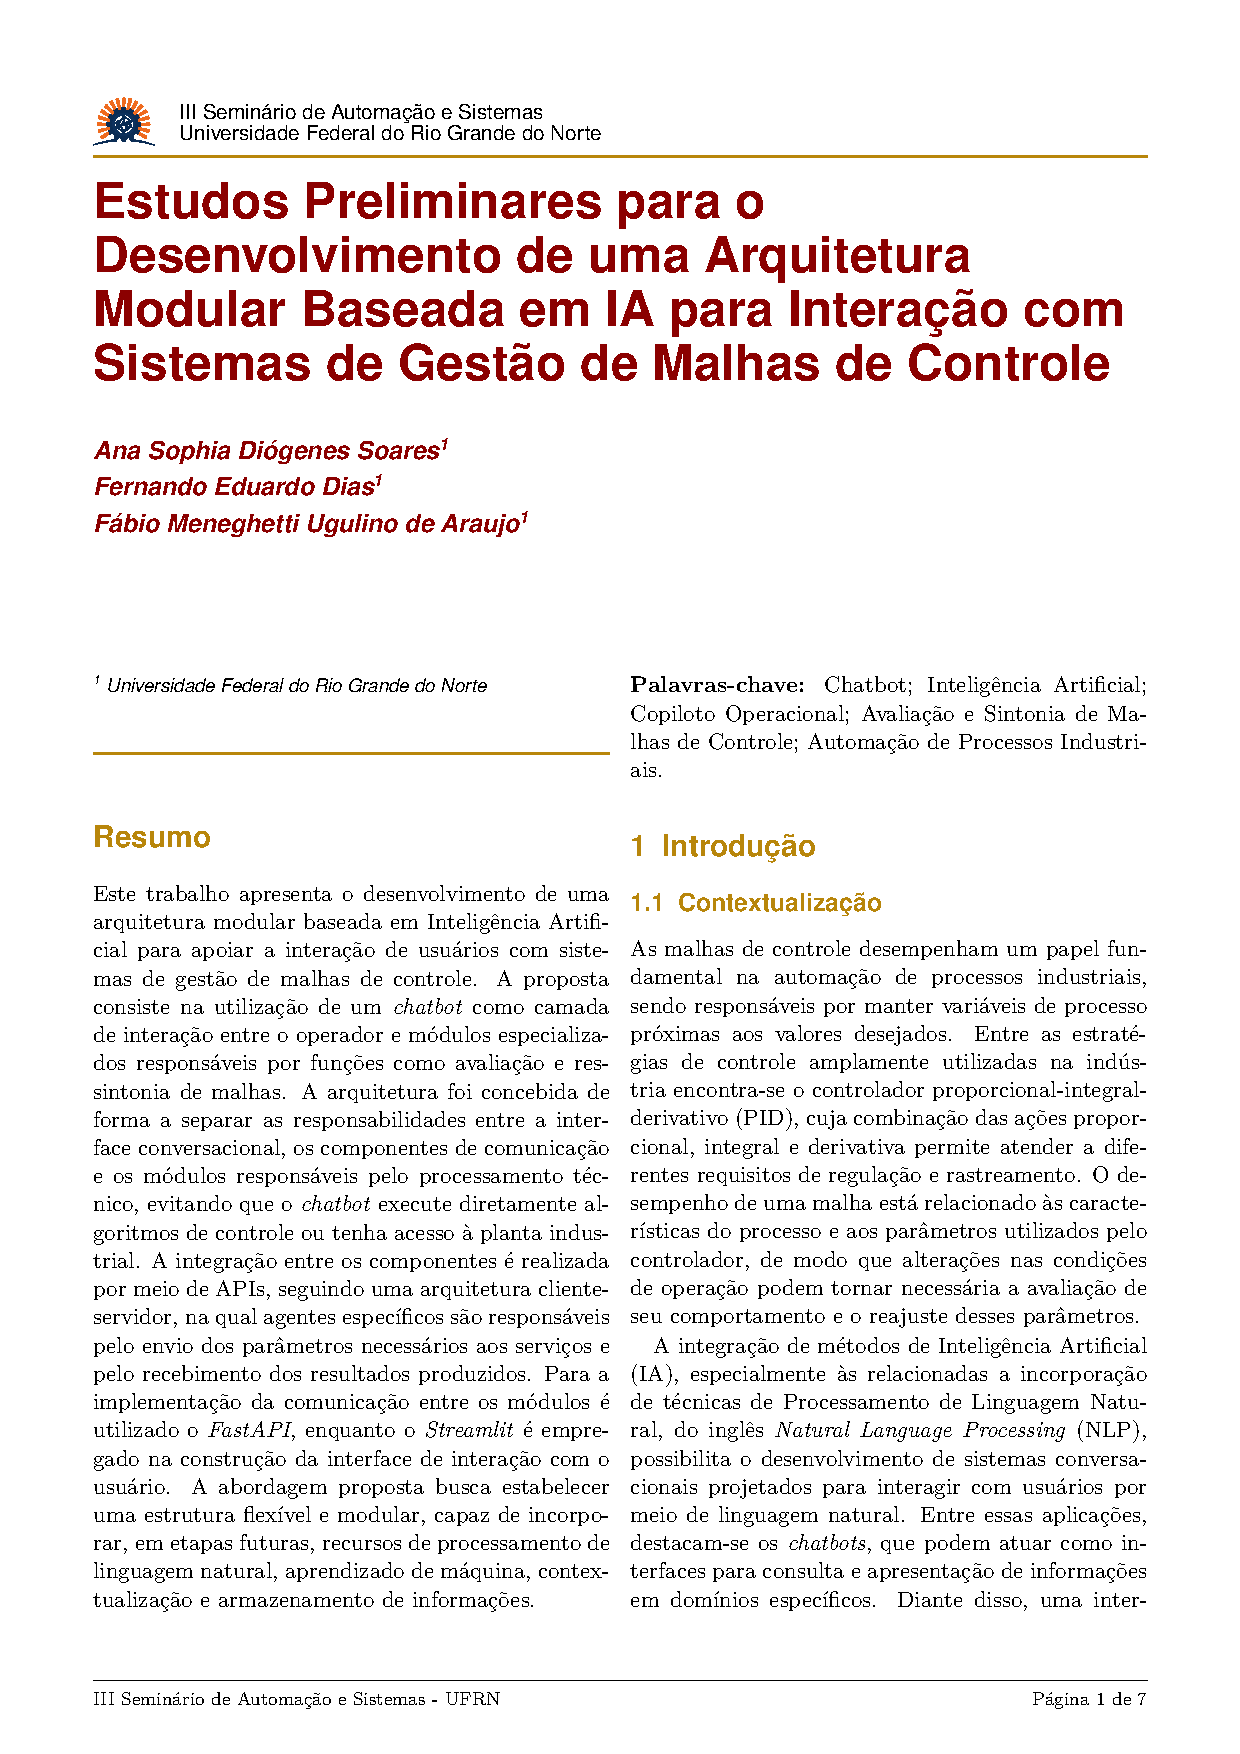
\includepdf[pages=-,fitpaper=A4]{artigos/01_estudos_preliminares_para_o_desenvolvimento_de_uma_arquitetura_modular_baseada_em_ia_para_interacao_com_sistemas_de_gestao_de_malhas_de_controle.pdf}
\addcontentsline{toc}{section}{Estudos preliminares para o desenvolvimento de uma arquitetura modular baseada em IA para interação com sistemas de gestão de malhas de controle}

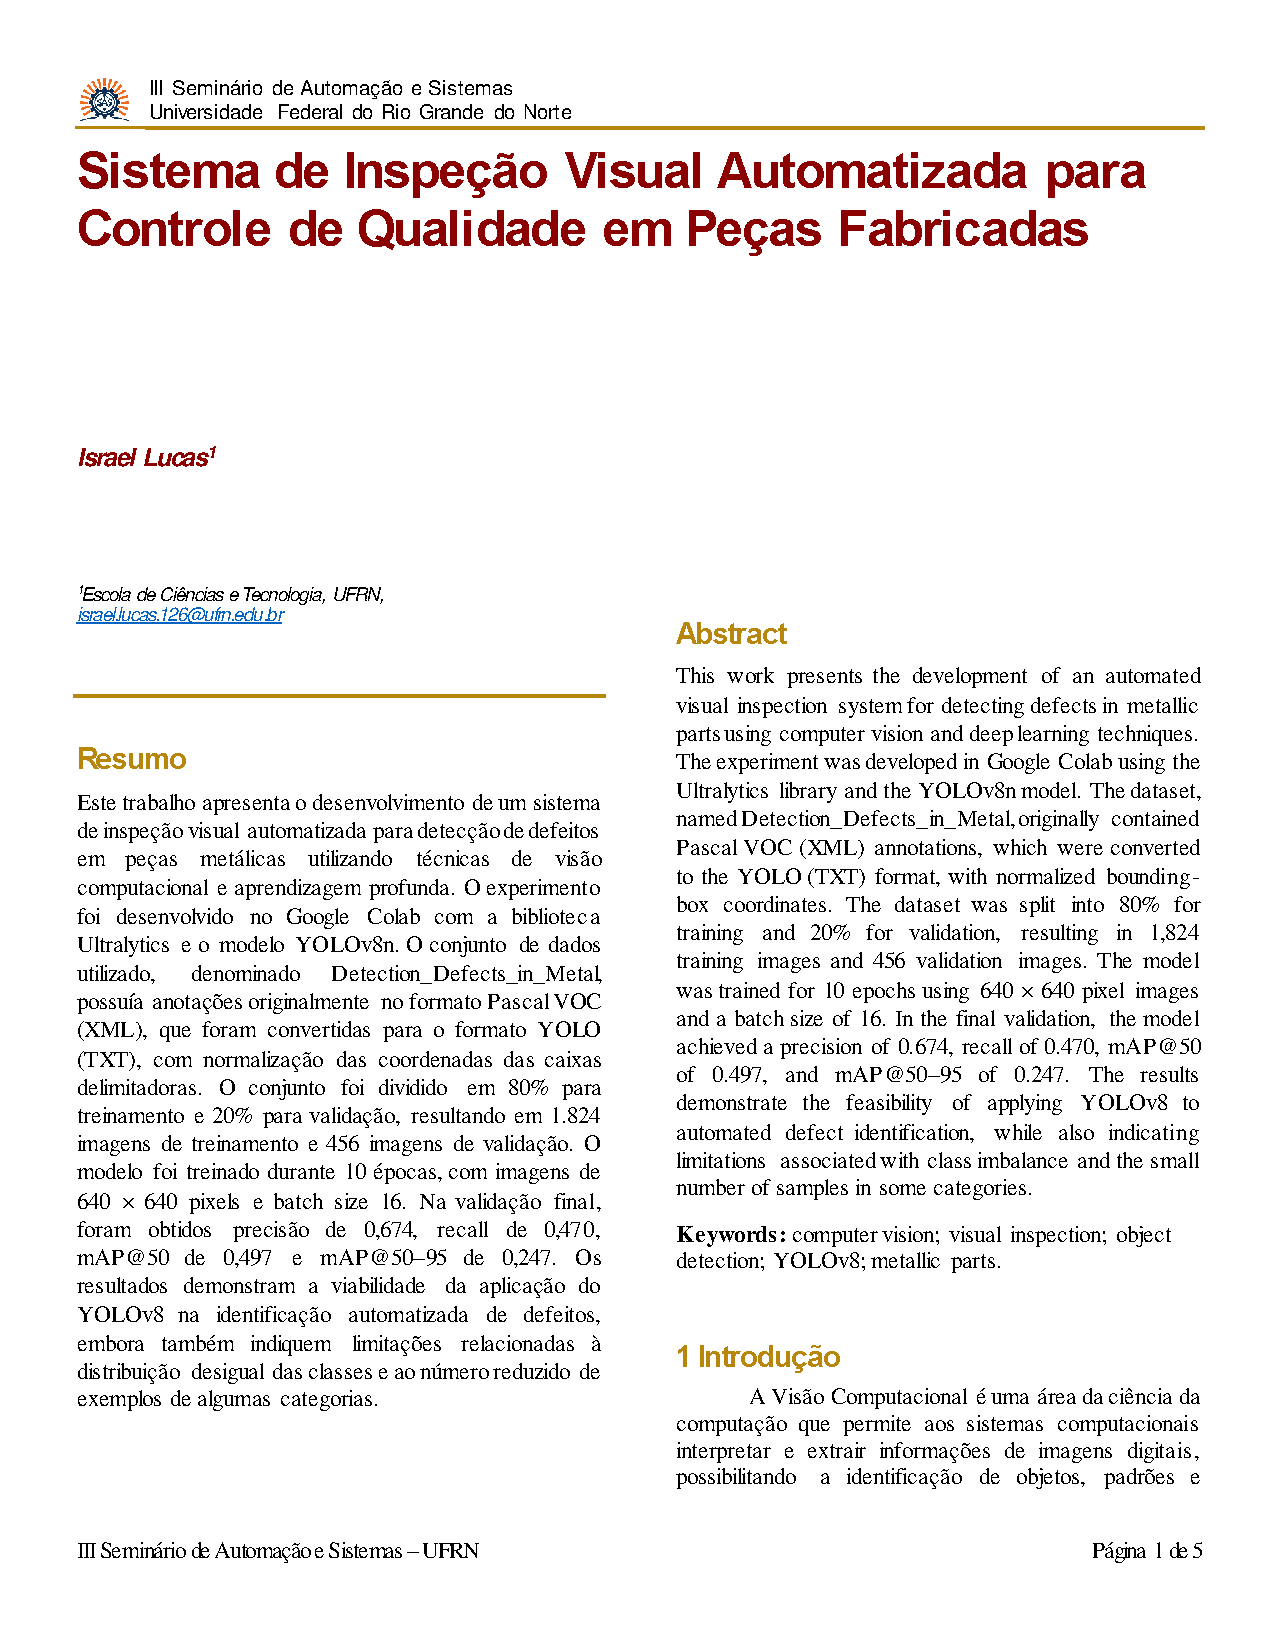
\includepdf[pages=-,fitpaper=A4]{artigos/02_sistema_de_inspecao_visual_automatizada_para_controle_de_qualidade_em_pecas_fabricadas.pdf}
\addcontentsline{toc}{section}{Sistema de inspeção visual automatizada para controle de qualidade em peças fabricadas}

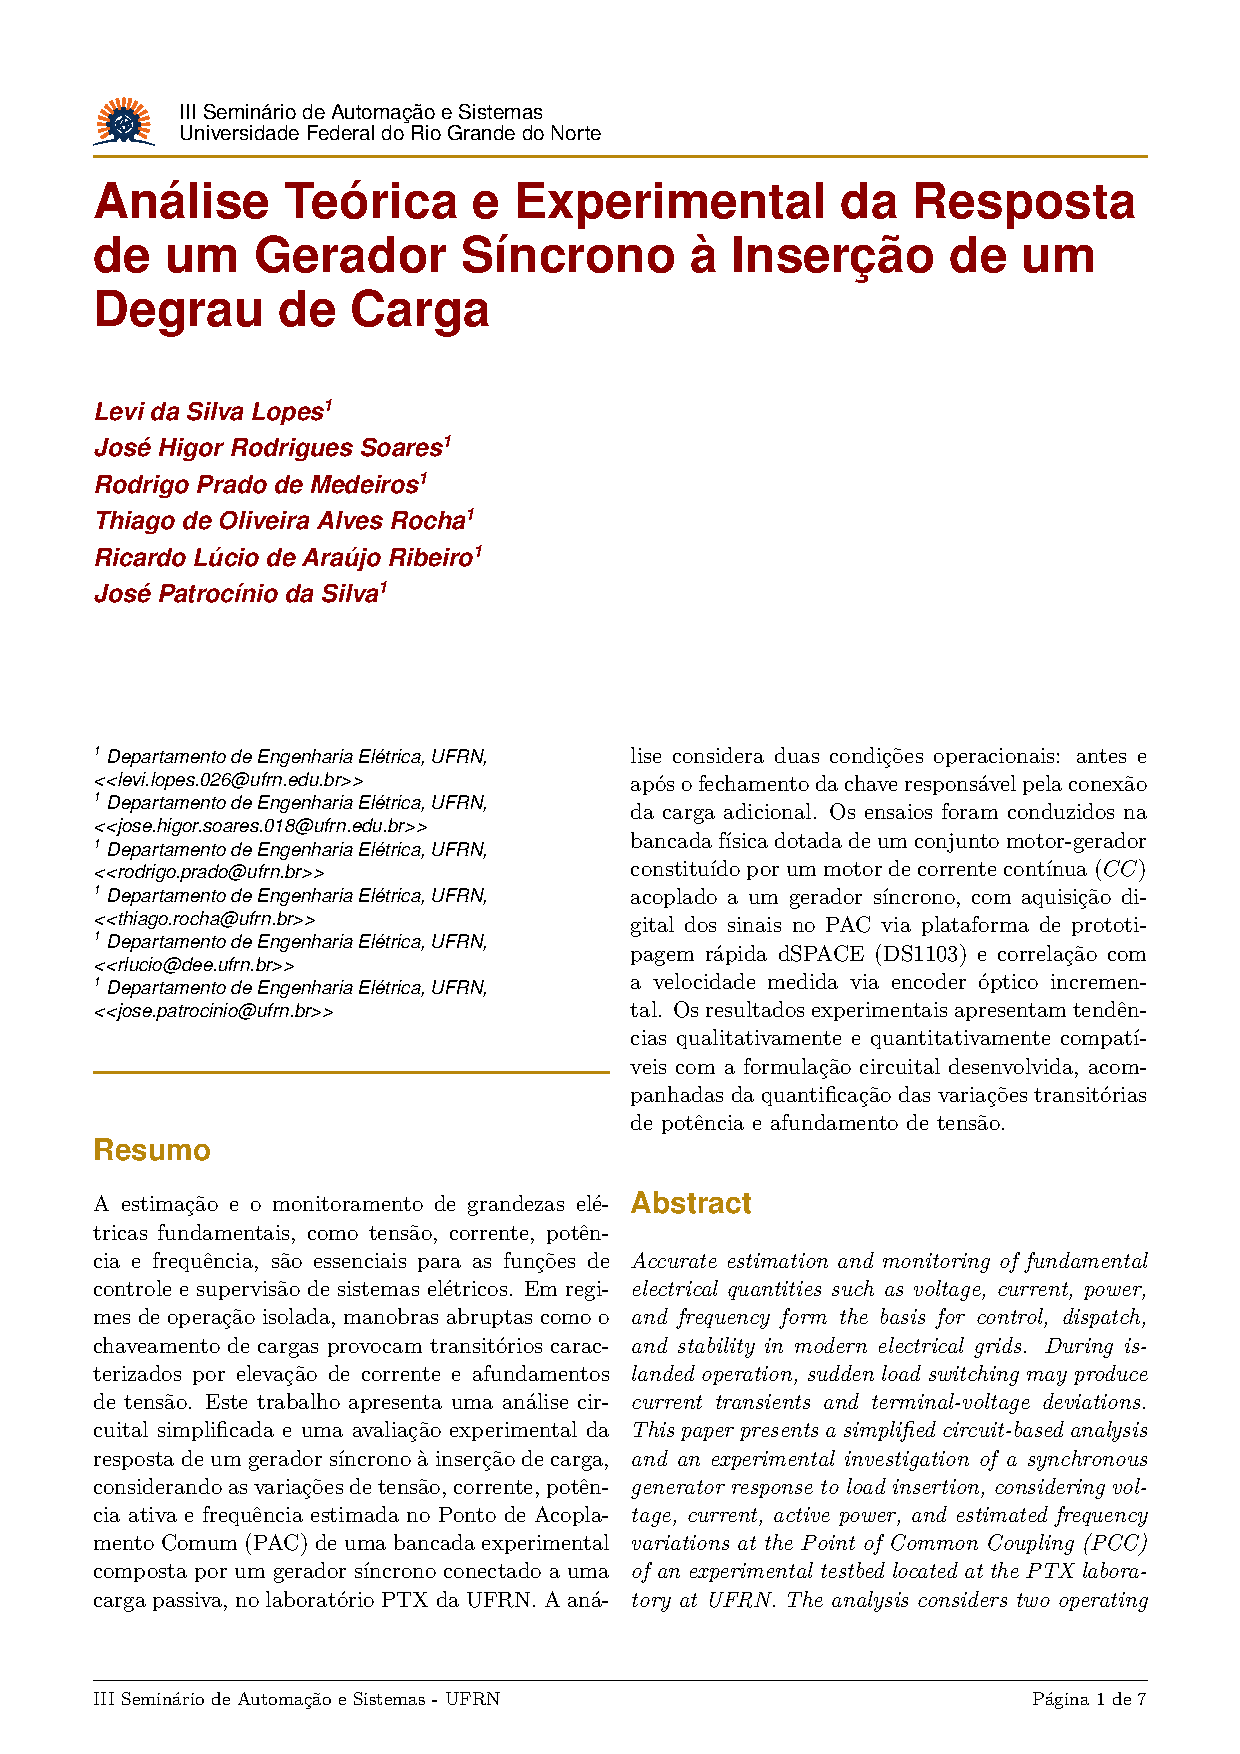
\includepdf[pages=-,fitpaper=A4]{artigos/03_analise_teorica_e_experimental_da_resposta_de_um_gerador_sincrono_a_insercao_de_um_degrau_de_carga.pdf}
\addcontentsline{toc}{section}{Análise teórica e experimental da resposta de um gerador síncrono à inserção de um degrau de carga}

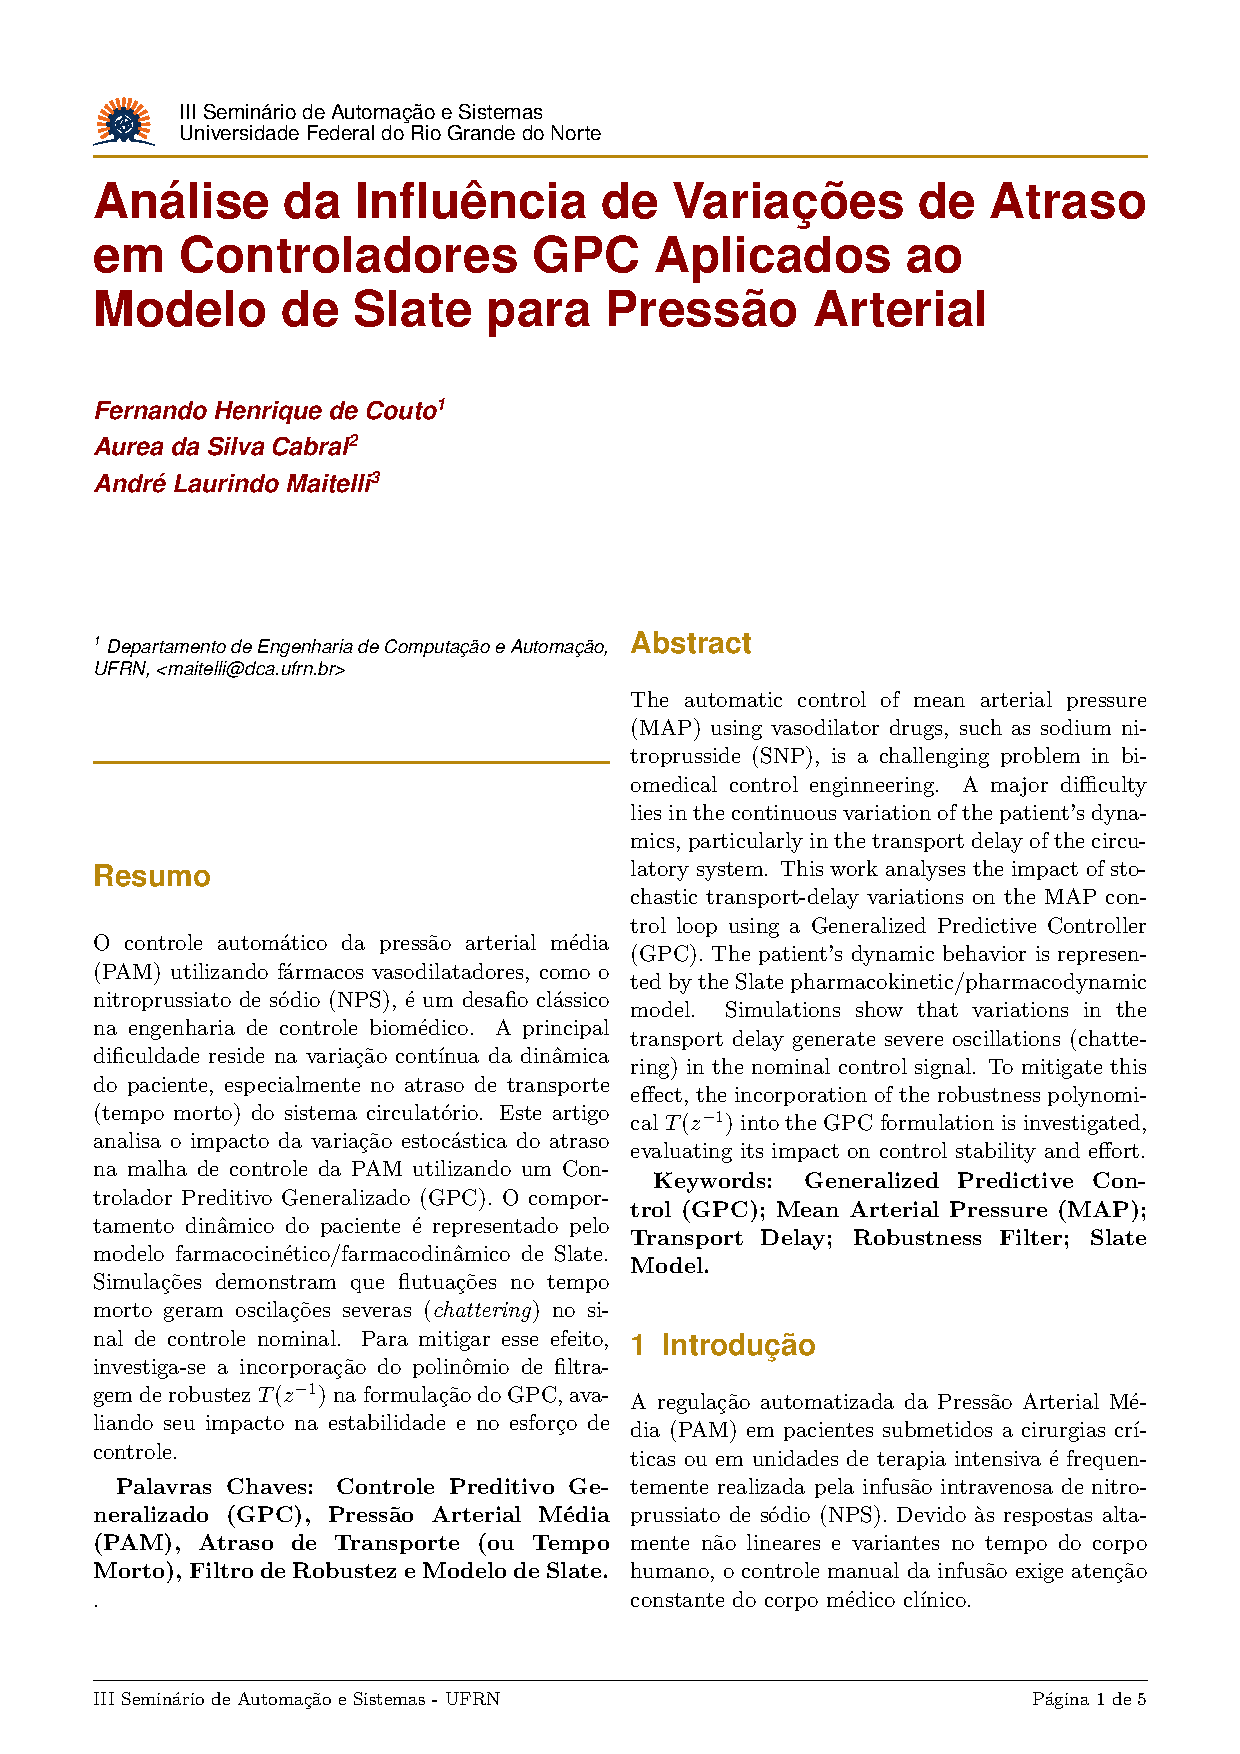
\includepdf[pages=-,fitpaper=A4]{artigos/04_analise_da_influencia_de_variacoes_de_atraso_em_controladores_gpc_aplicados_ao_modelo_de_slate_para_pressao_arterial.pdf}
\addcontentsline{toc}{section}{Análise da influência de variações de atraso em controladores GPC aplicados ao modelo de slate para pressão arterial}

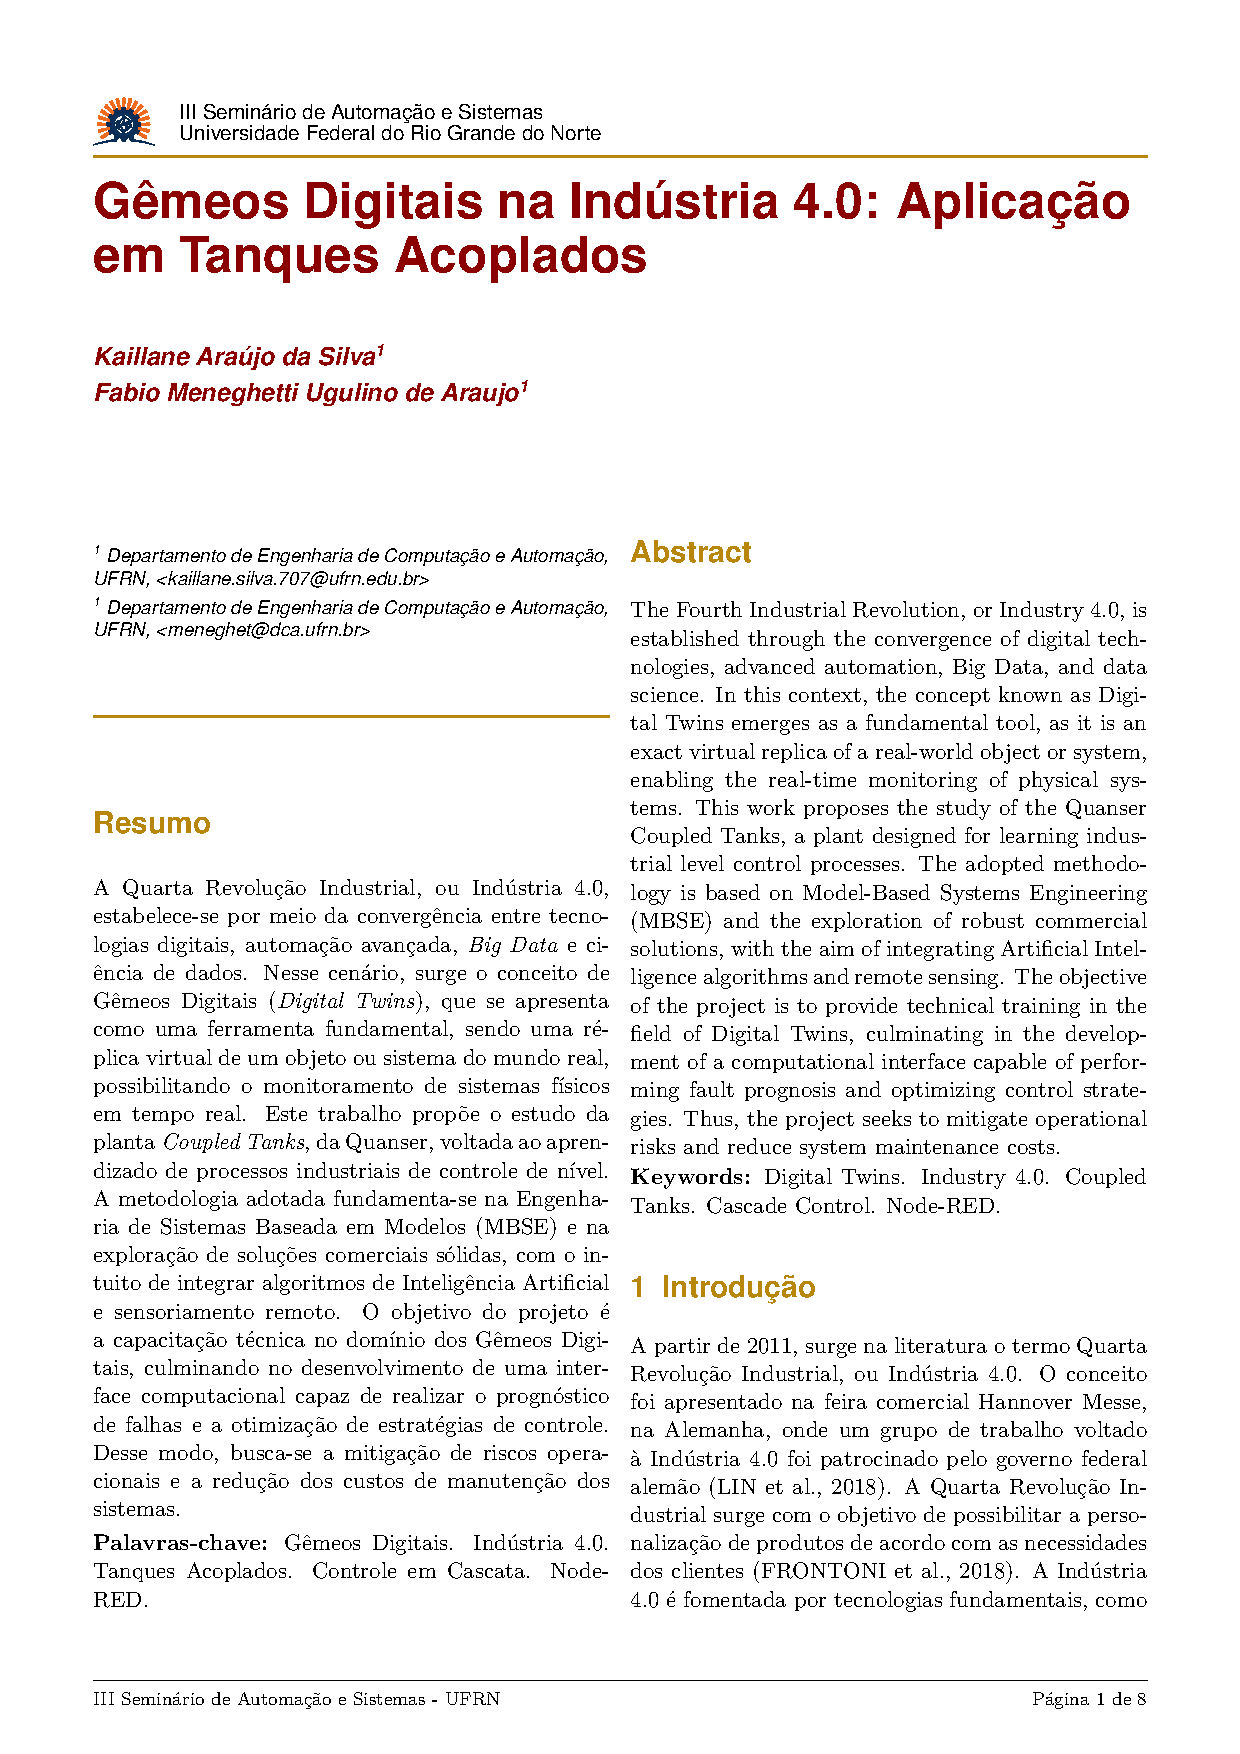
\includepdf[pages=-,fitpaper=A4]{artigos/05_gemeos_digitais_na_industria_4_0_aplicacao_em_tanques_acoplados.pdf}
\addcontentsline{toc}{section}{Gêmeos digitais na indústria 4.0: aplicação em tanques acoplados}

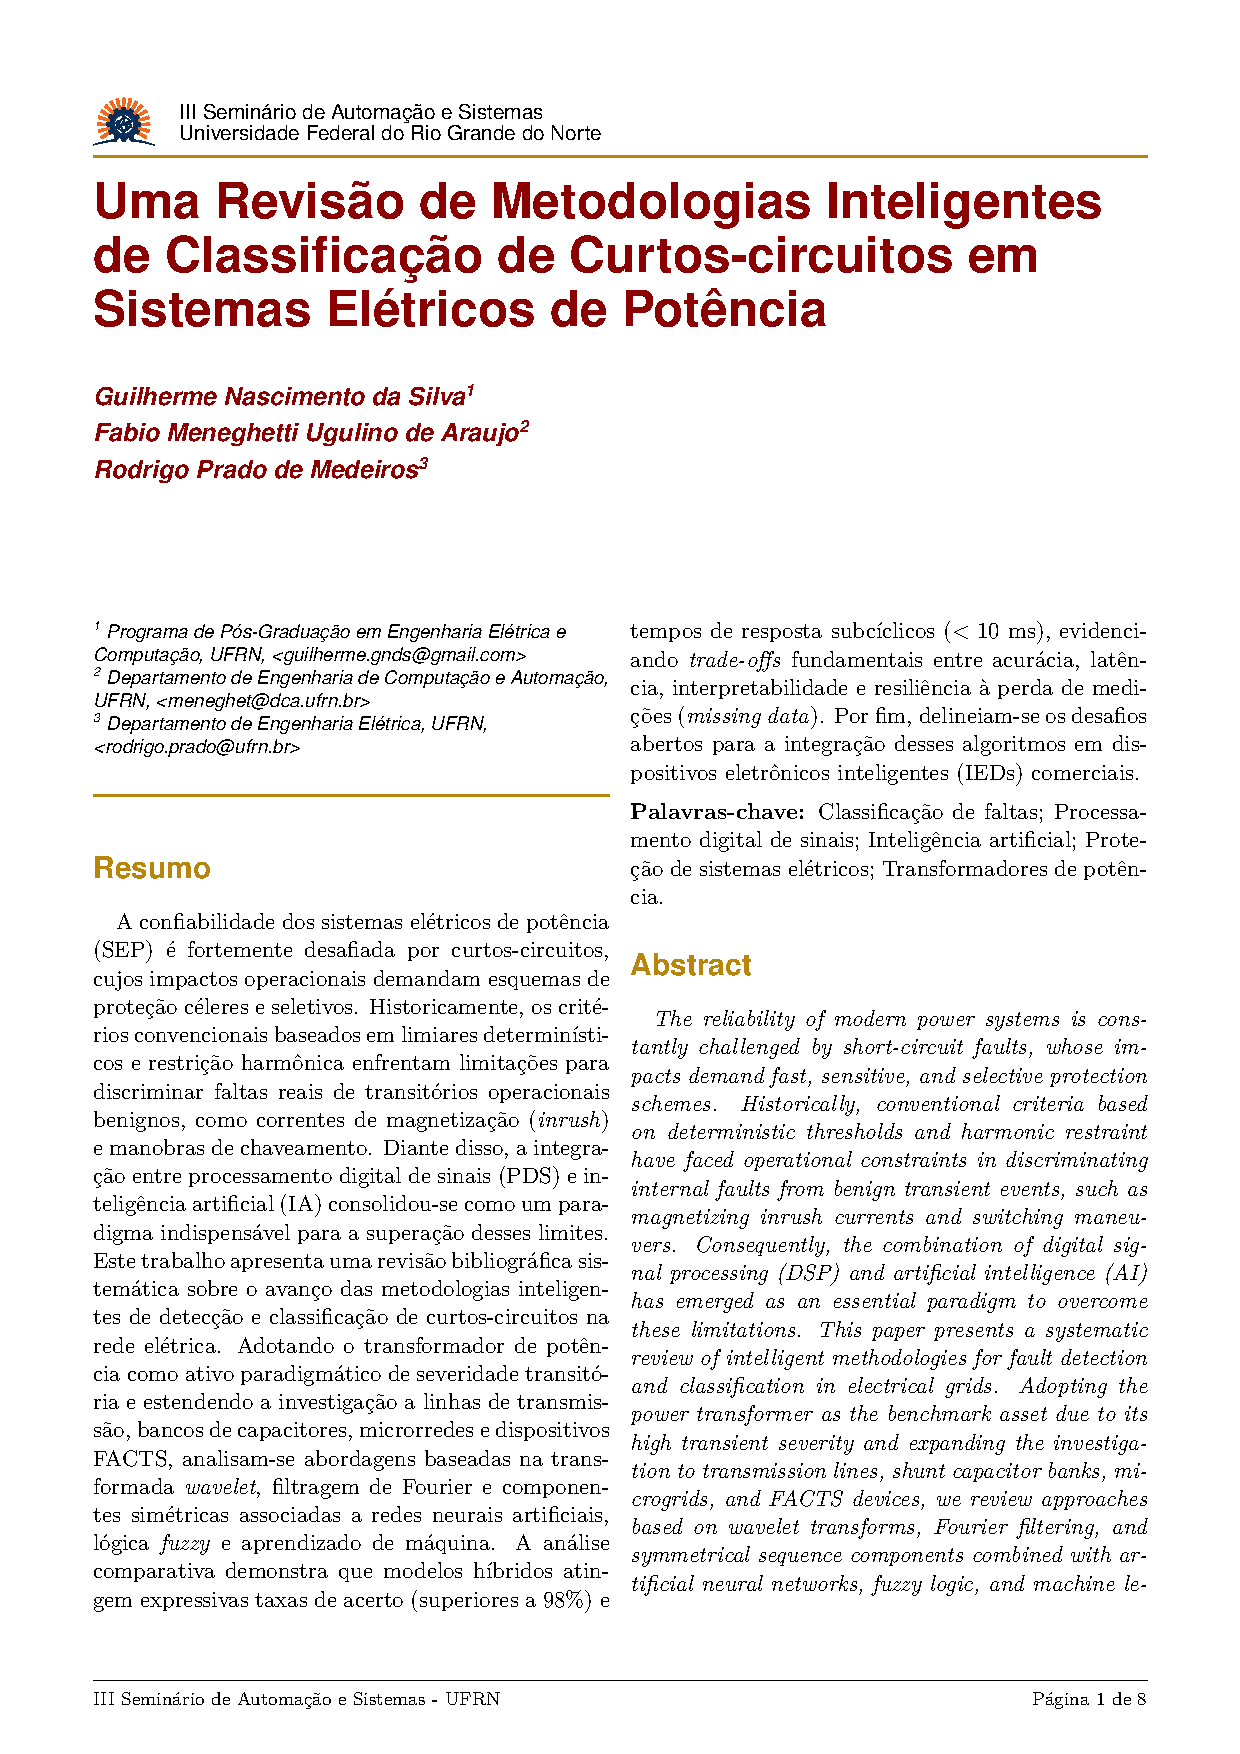
\includepdf[pages=-,fitpaper=A4]{artigos/06_uma_revisao_de_metodologias_inteligentes_de_classificacao_de_curtos_circuitos_em_sistemas_eletricos_de_potencia.pdf}
\addcontentsline{toc}{section}{Uma revisão de metodologias inteligentes de classificação de curtos circuitos em sistemas elétricos de potência}

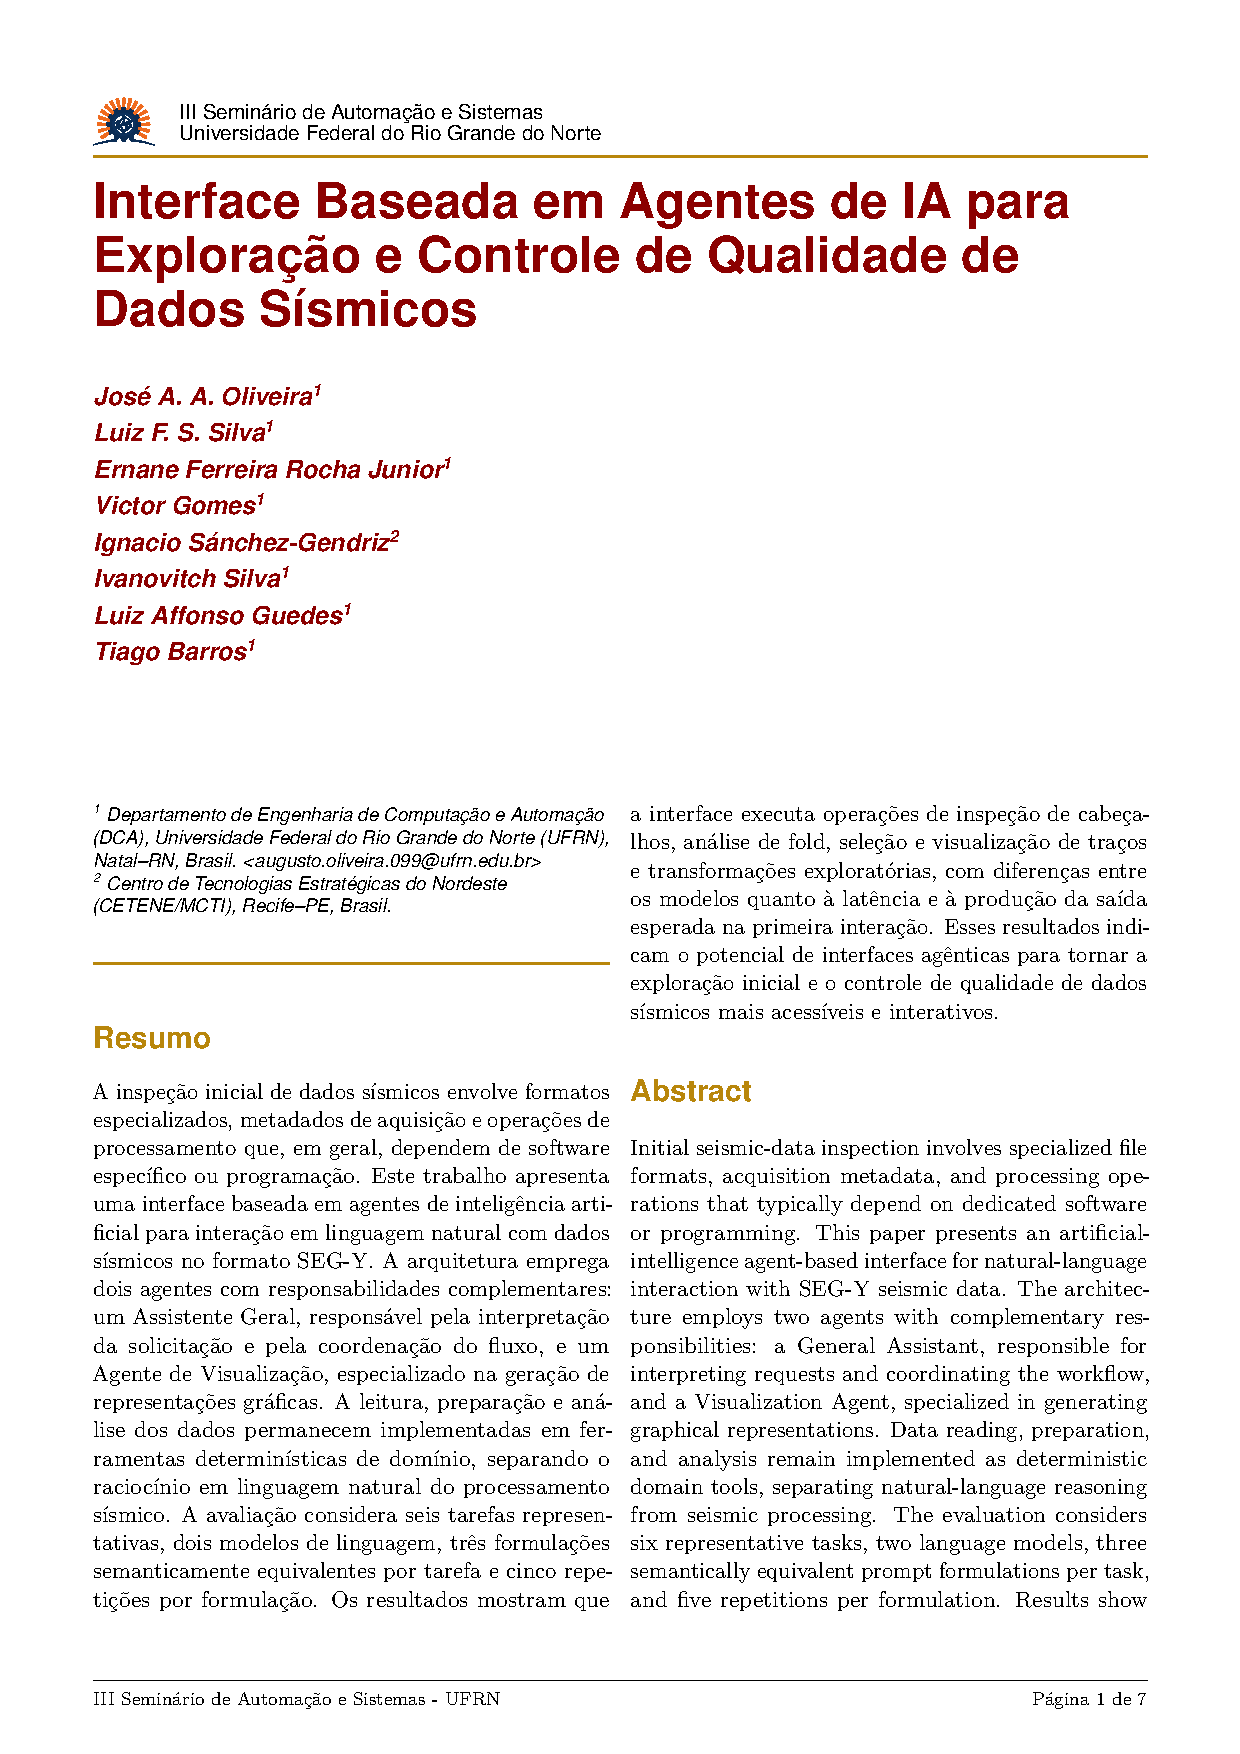
\includepdf[pages=-,fitpaper=A4]{artigos/07_interface_baseada_em_agentes_de_ia_para_exploracao_e_controle_de_qualidade_de_dados_sismicos.pdf}
\addcontentsline{toc}{section}{Interface baseada em agentes de IA para exploração e controle de qualidade de dados sísmicos}

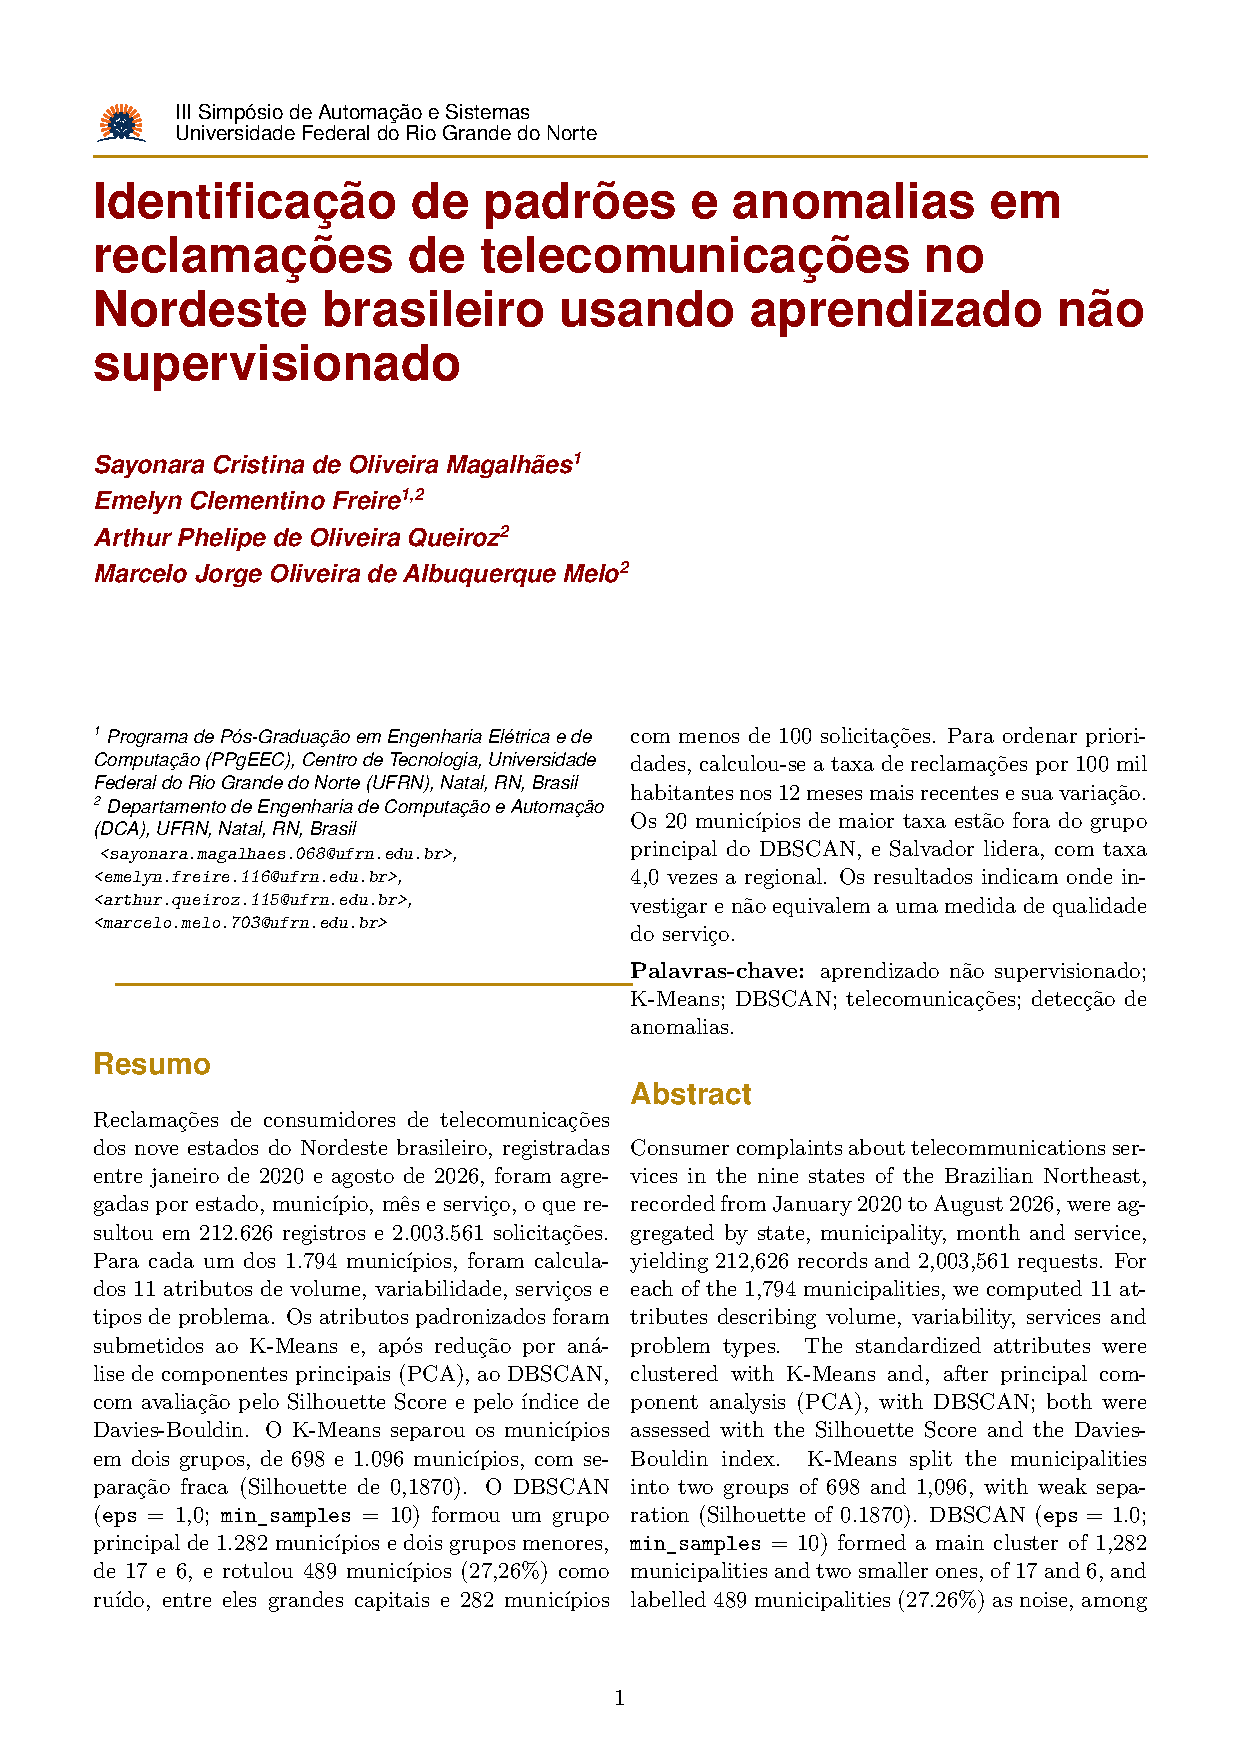
\includepdf[pages=-,fitpaper=A4]{artigos/08_identificacao_de_padroes_e_anomalias_em_reclamacoes_de_telecomunicacoes_no_nordeste_brasileiro_usando_aprendizado_nao_supervisionado.pdf}
\addcontentsline{toc}{section}{Identificação de padrões e anomalias em reclamações de telecomunicações no Nordeste brasileiro usando aprendizado não supervisionado}

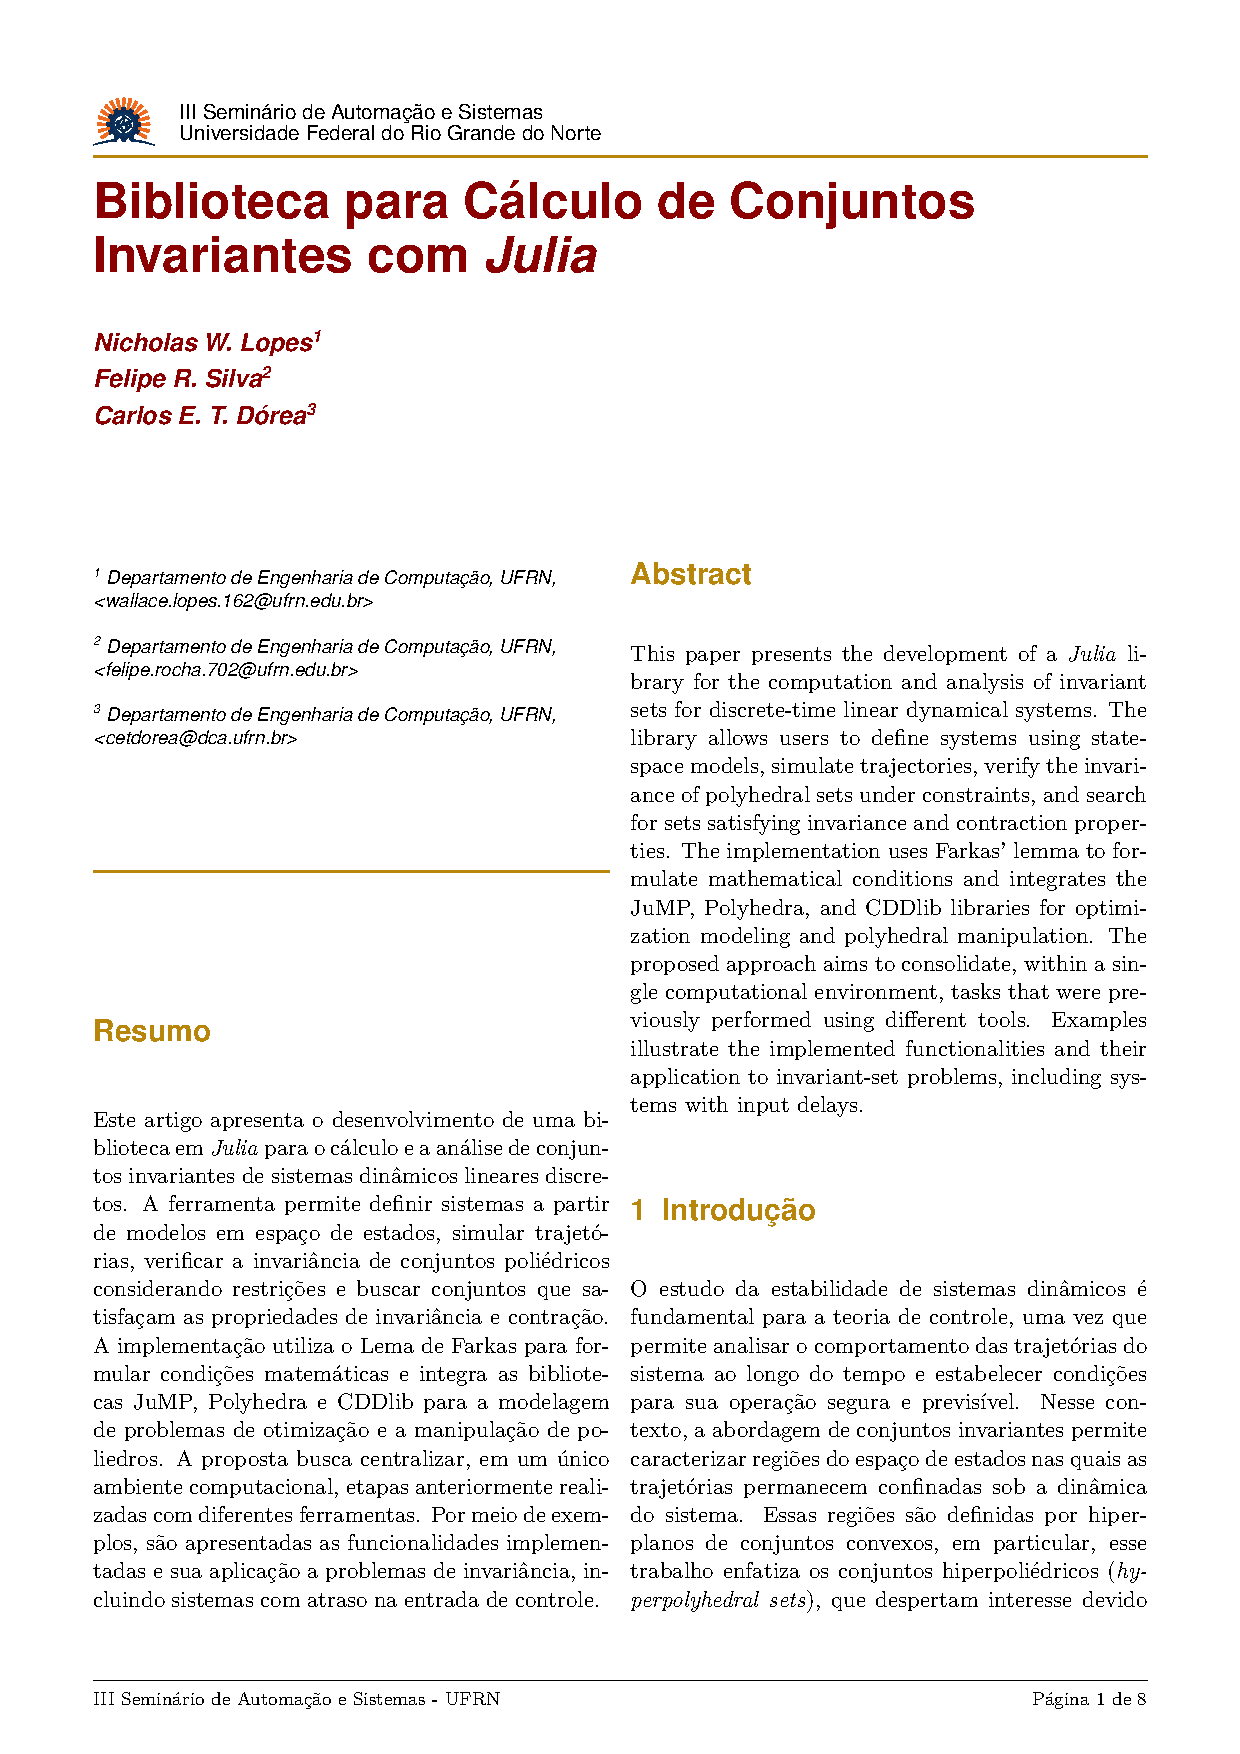
\includepdf[pages=-,fitpaper=A4]{artigos/10_biblioteca_para_calculo_de_conjuntos_invariantes_com_julia.pdf}
\addcontentsline{toc}{section}{Biblioteca para cálculo de conjuntos invariantes com Julia}

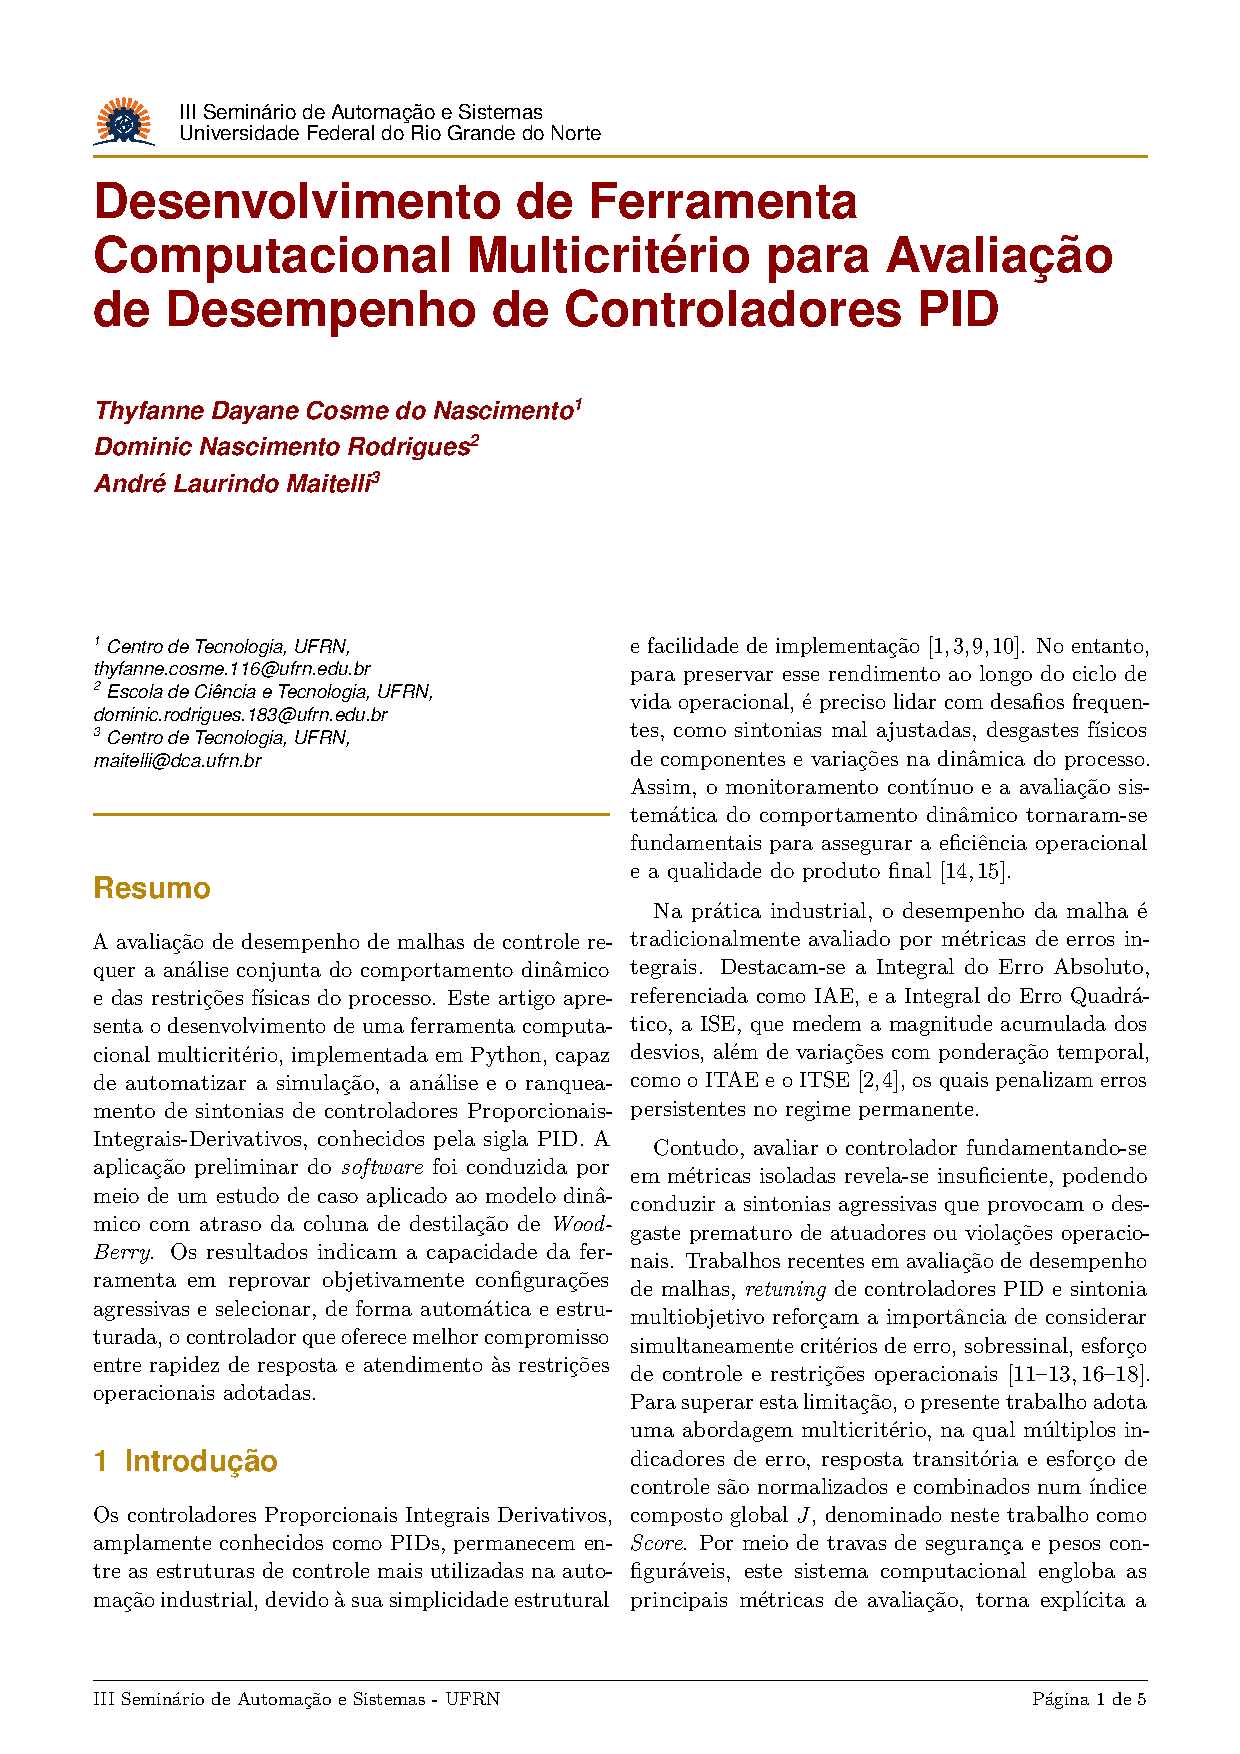
\includepdf[pages=-,fitpaper=A4]{artigos/12_desenvolvimento_de_ferramenta_computacional_multicriterio_para_avaliacao_de_desempenho_de_controladores_pid.pdf}
\addcontentsline{toc}{section}{Desenvolvimento de uma ferramenta computacional multicritério para avaliação de desempenho de controladores PID}

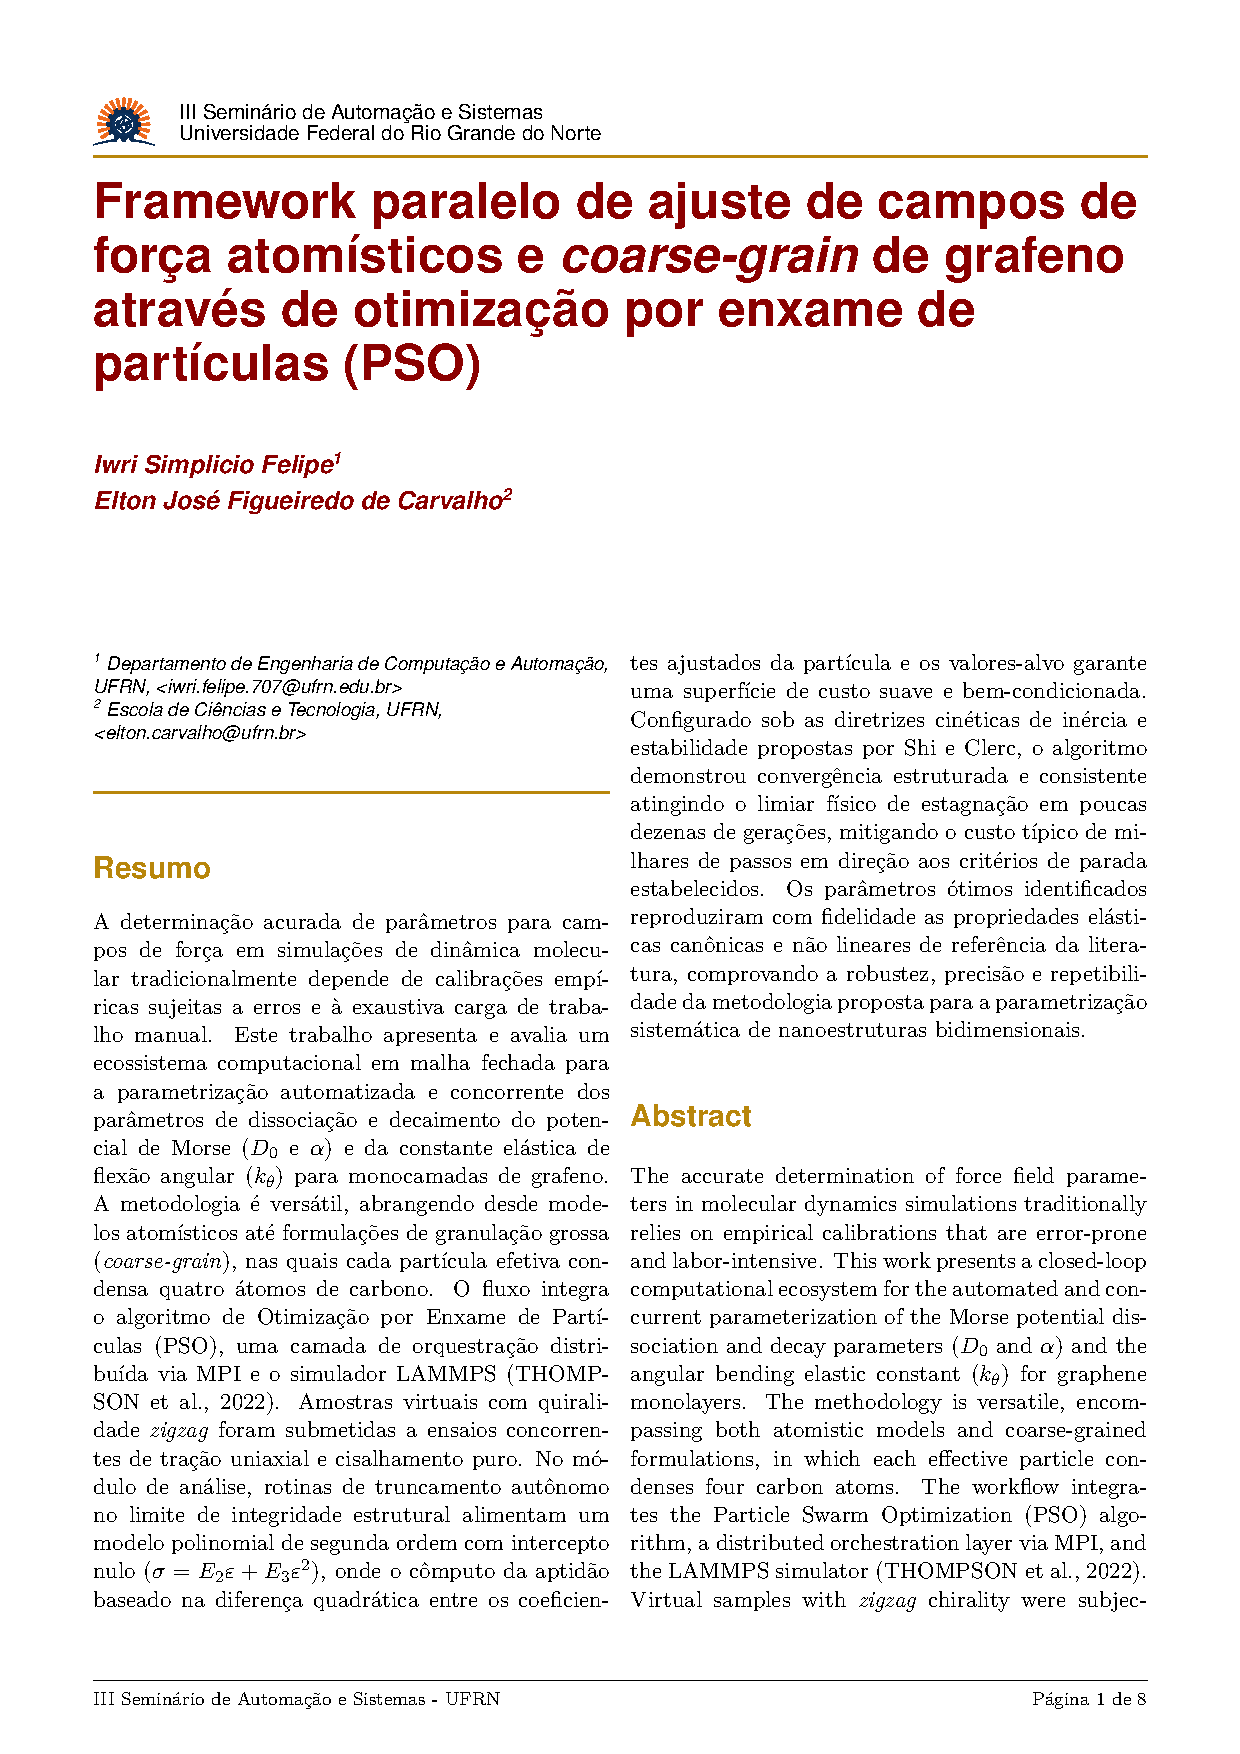
\includepdf[pages=-,fitpaper=A4]{artigos/13_framework_paralelo_de_ajuste_de_campos_de_forca_atomisticos_e_coarse_grain_de_grafeno_atraves_de_otimizacao_por_enxame_de_particulas_pso.pdf}
\addcontentsline{toc}{section}{Framework paralelo de ajuste de campos de força atomísticos e coarse-grain de grafeno através de otimização por enxame de partículas PSO}

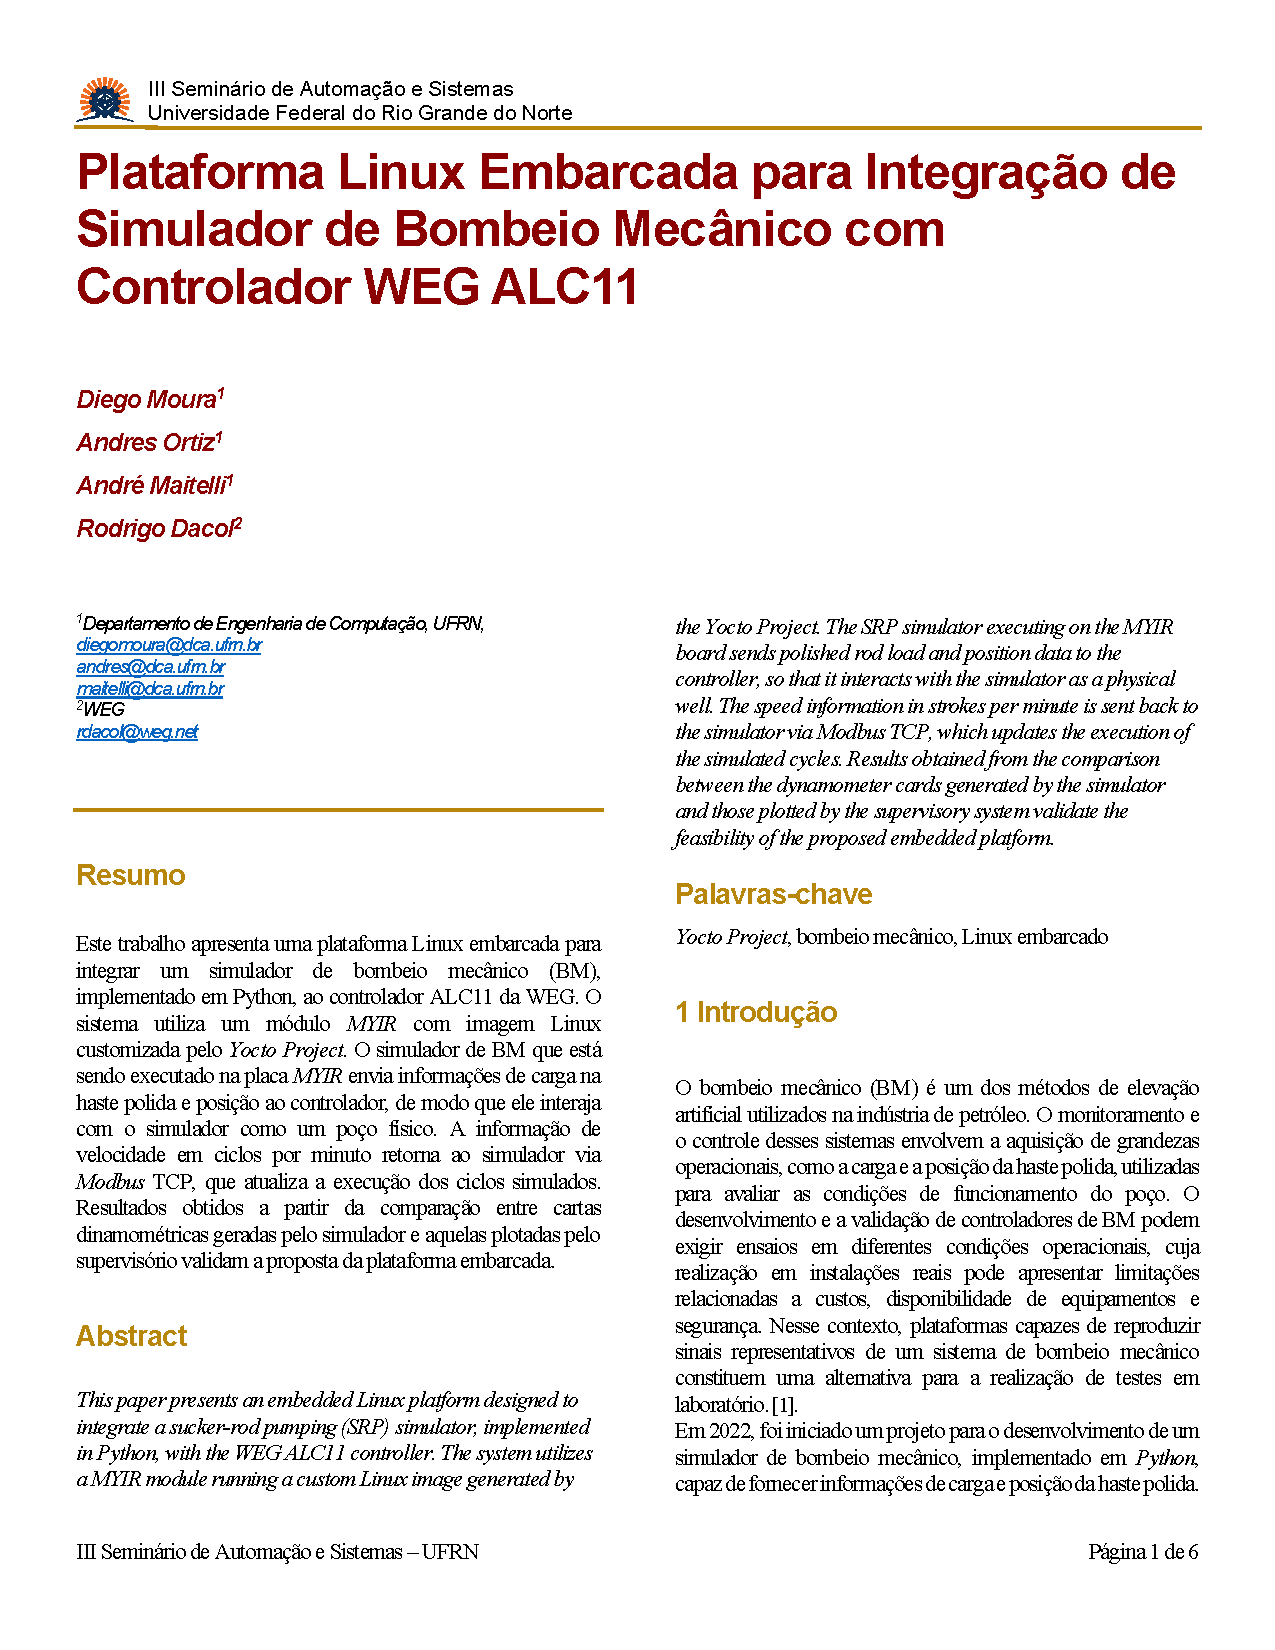
\includepdf[pages=-,fitpaper=A4]{artigos/14_plataforma_linux_embarcada_para_integracao_de_simulador_de_bombeio_mecanico_com_controlador_weg_alc11.pdf}
\addcontentsline{toc}{section}{Plataforma Linux embarcada para integração de simulador de bombeio mecânico com controlador WEG ALC11}

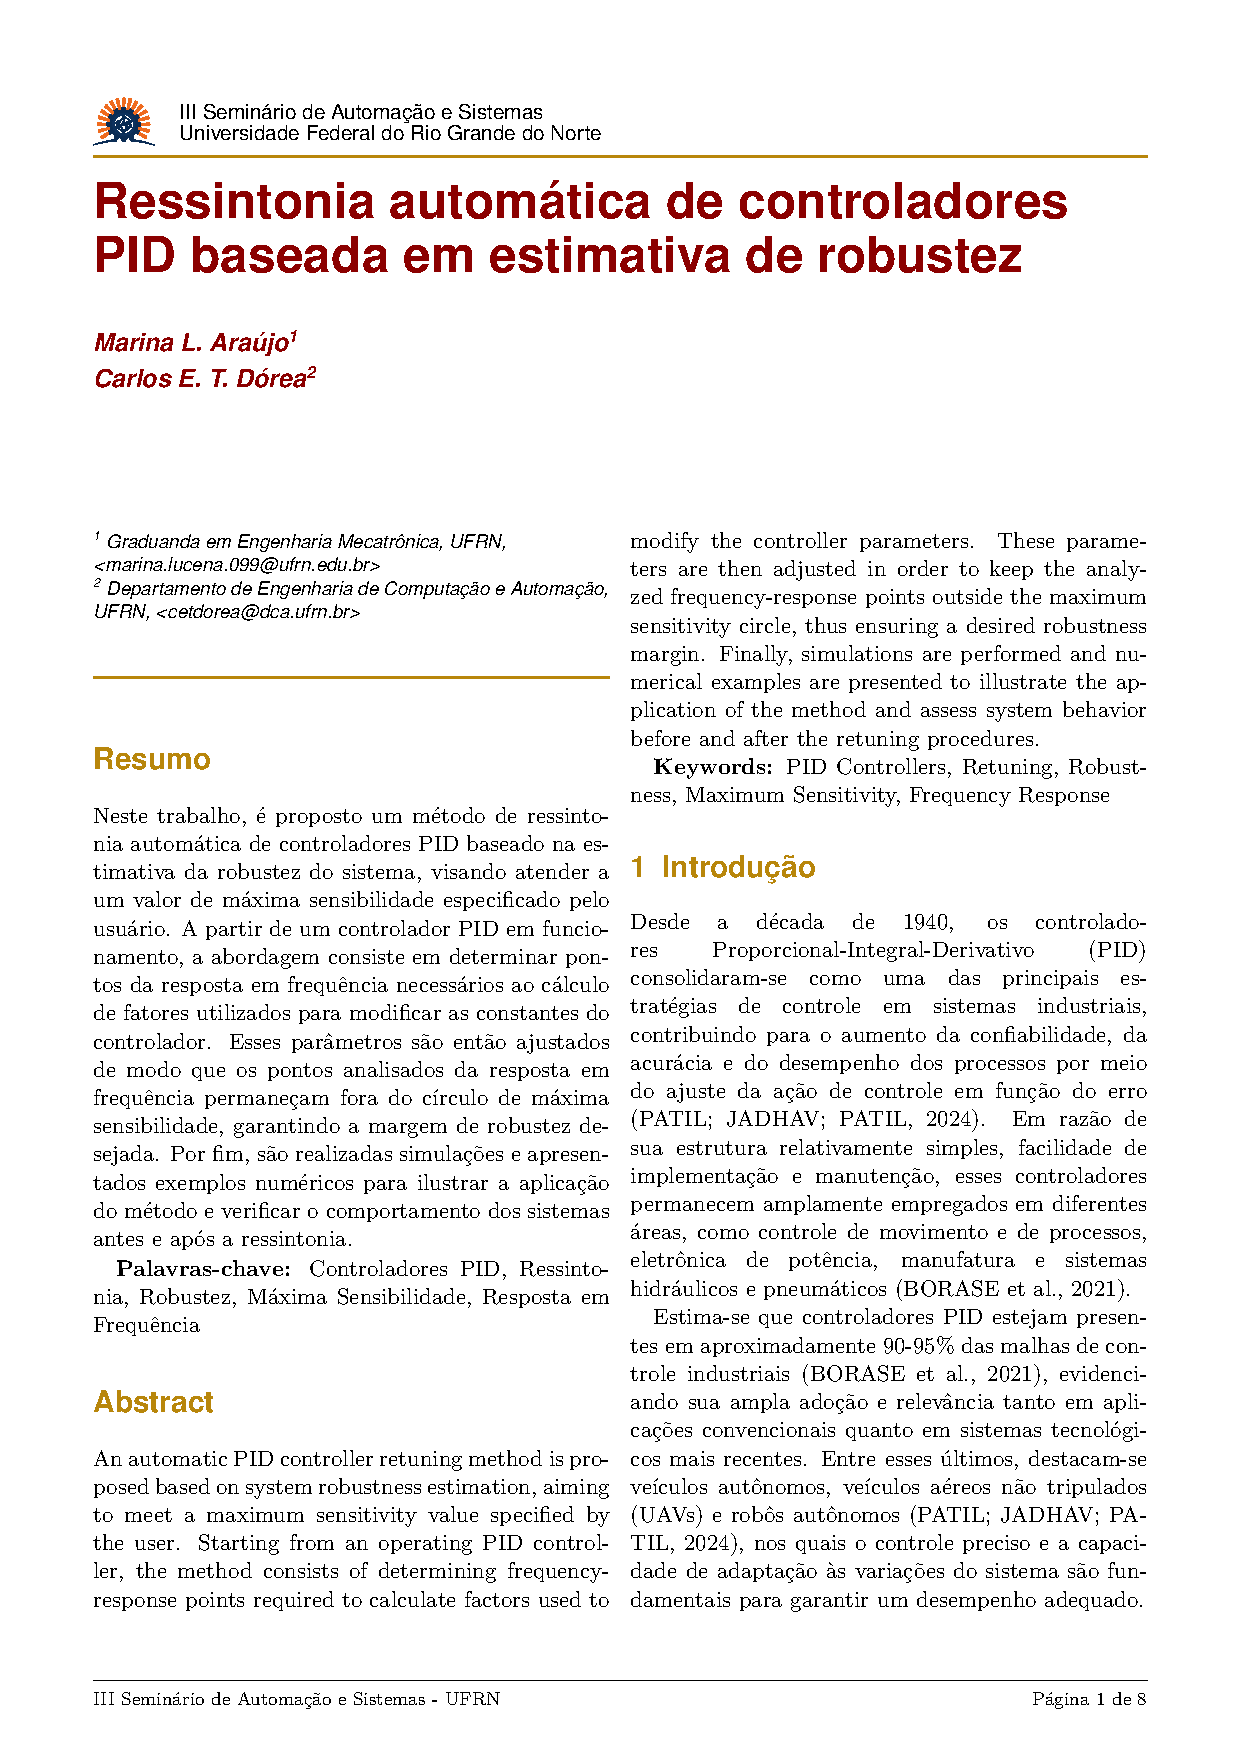
\includepdf[pages=-,fitpaper=A4]{artigos/15_ressintonia_automatica_de_controladores_pid_baseada_em_estimativa_de_robustez.pdf}
\addcontentsline{toc}{section}{Ressintonia automática de controladores PID baseada em estimativa de robustez}

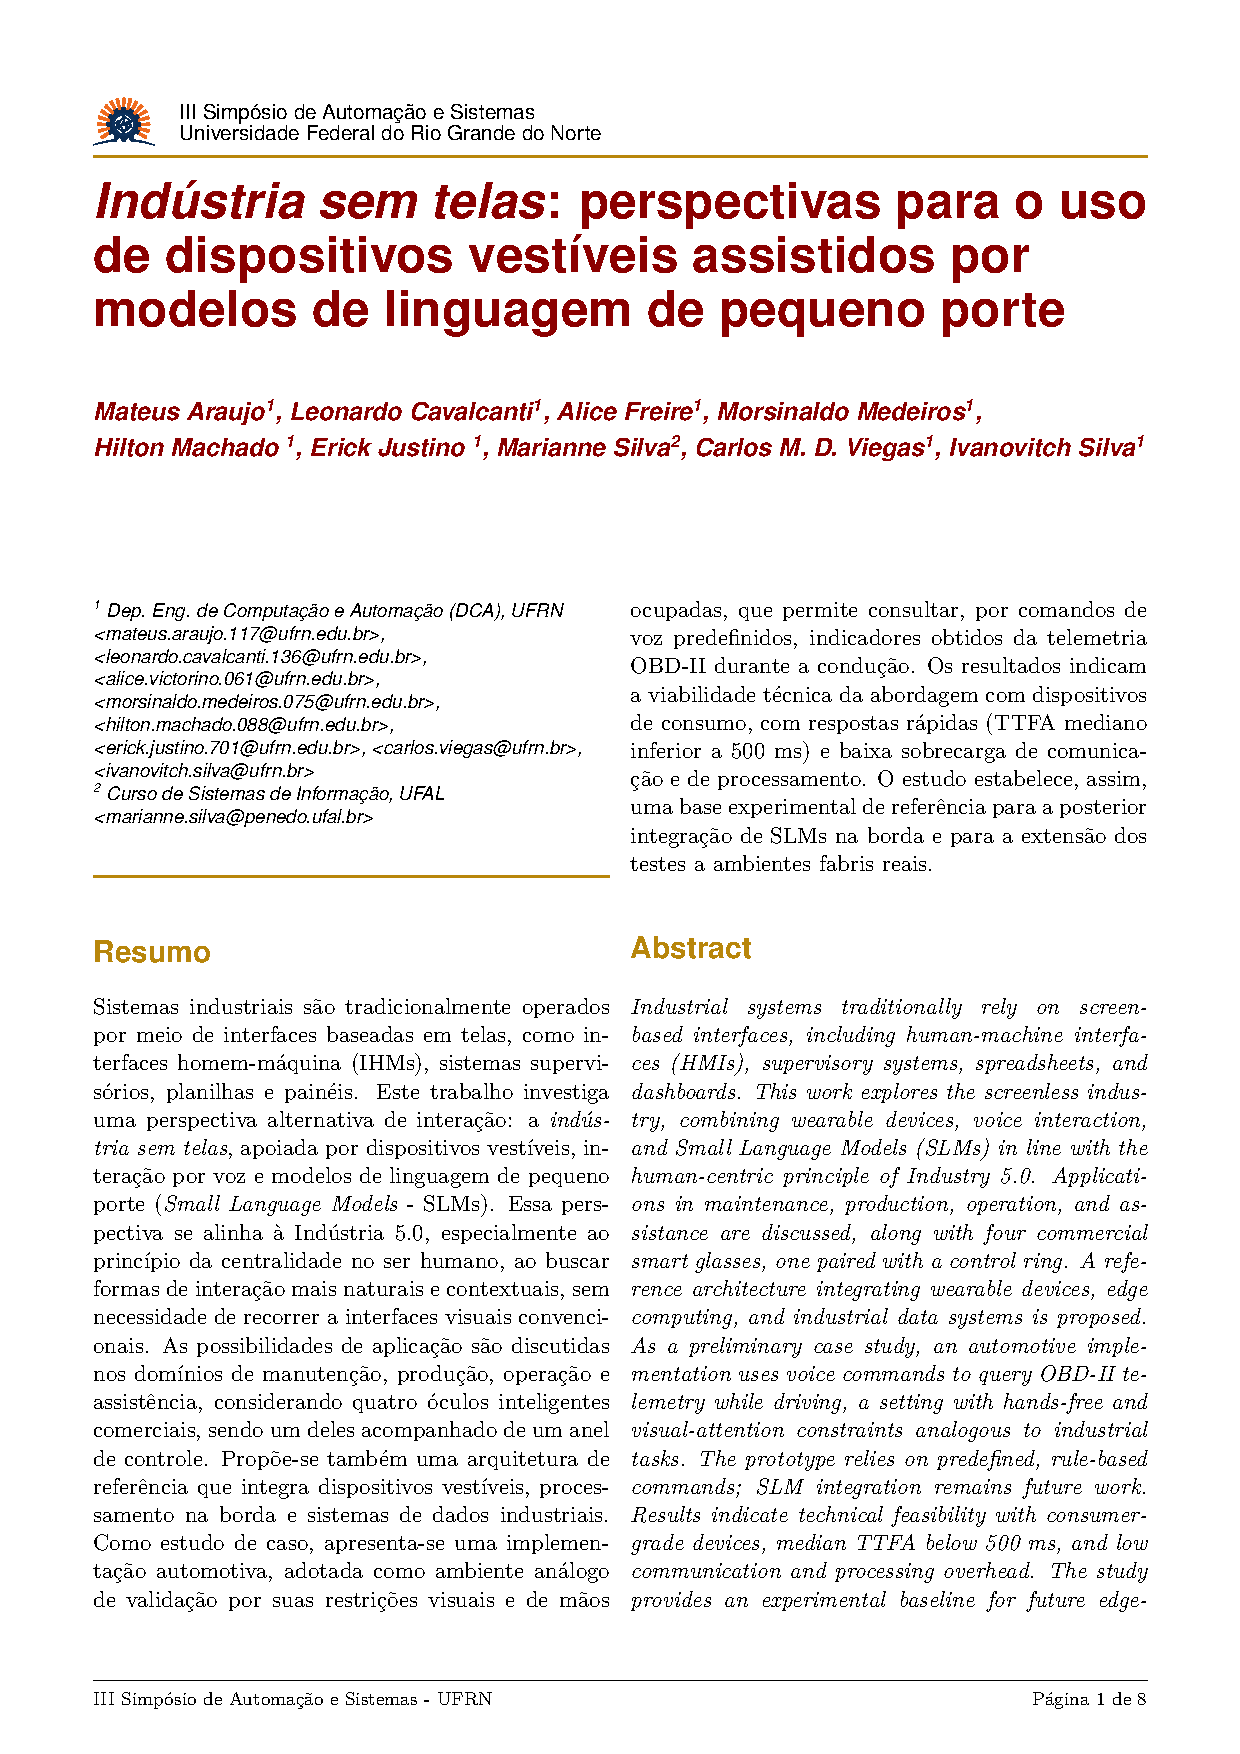
\includepdf[pages=-,fitpaper=A4]{artigos/16_industria_sem_telas_perspectivas_para_o_uso_de_dispositivos_vestiveis_assistidos_por_modelos_de_linguagem_de_pequeno_porte.pdf}
\addcontentsline{toc}{section}{Indústria sem telas: perspectivas para o uso de dispositivos vestíveis assistidos por modelos de linguagem de pequeno porte}

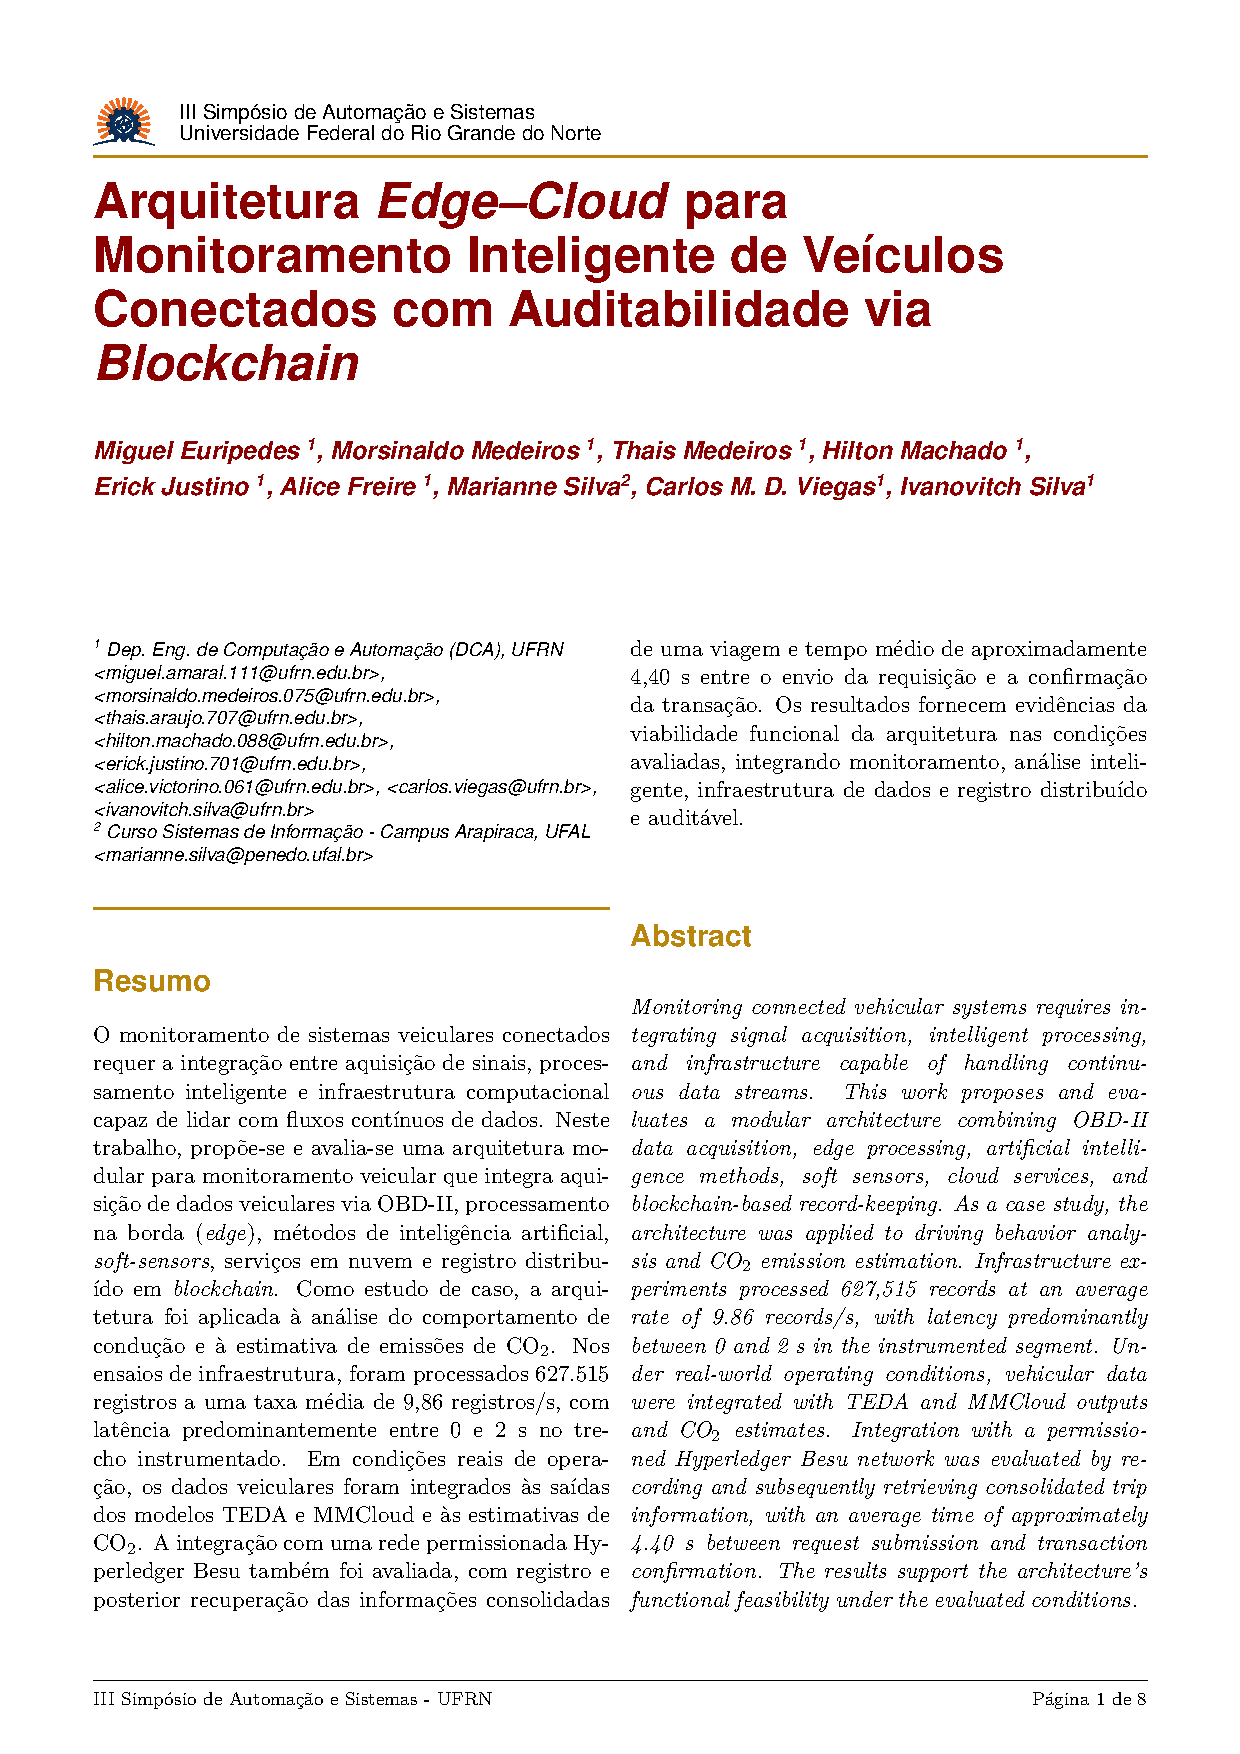
\includepdf[pages=-,fitpaper=A4]{artigos/17_arquitetura_edgecloud_para_monitoramento_inteligente_de_veiculos_conectados_com_auditabilidade_via_blockchain.pdf}
\addcontentsline{toc}{section}{Arquitetura edge-cloud para monitoramento inteligente de veículos conectados com auditabilidade via blockchain}

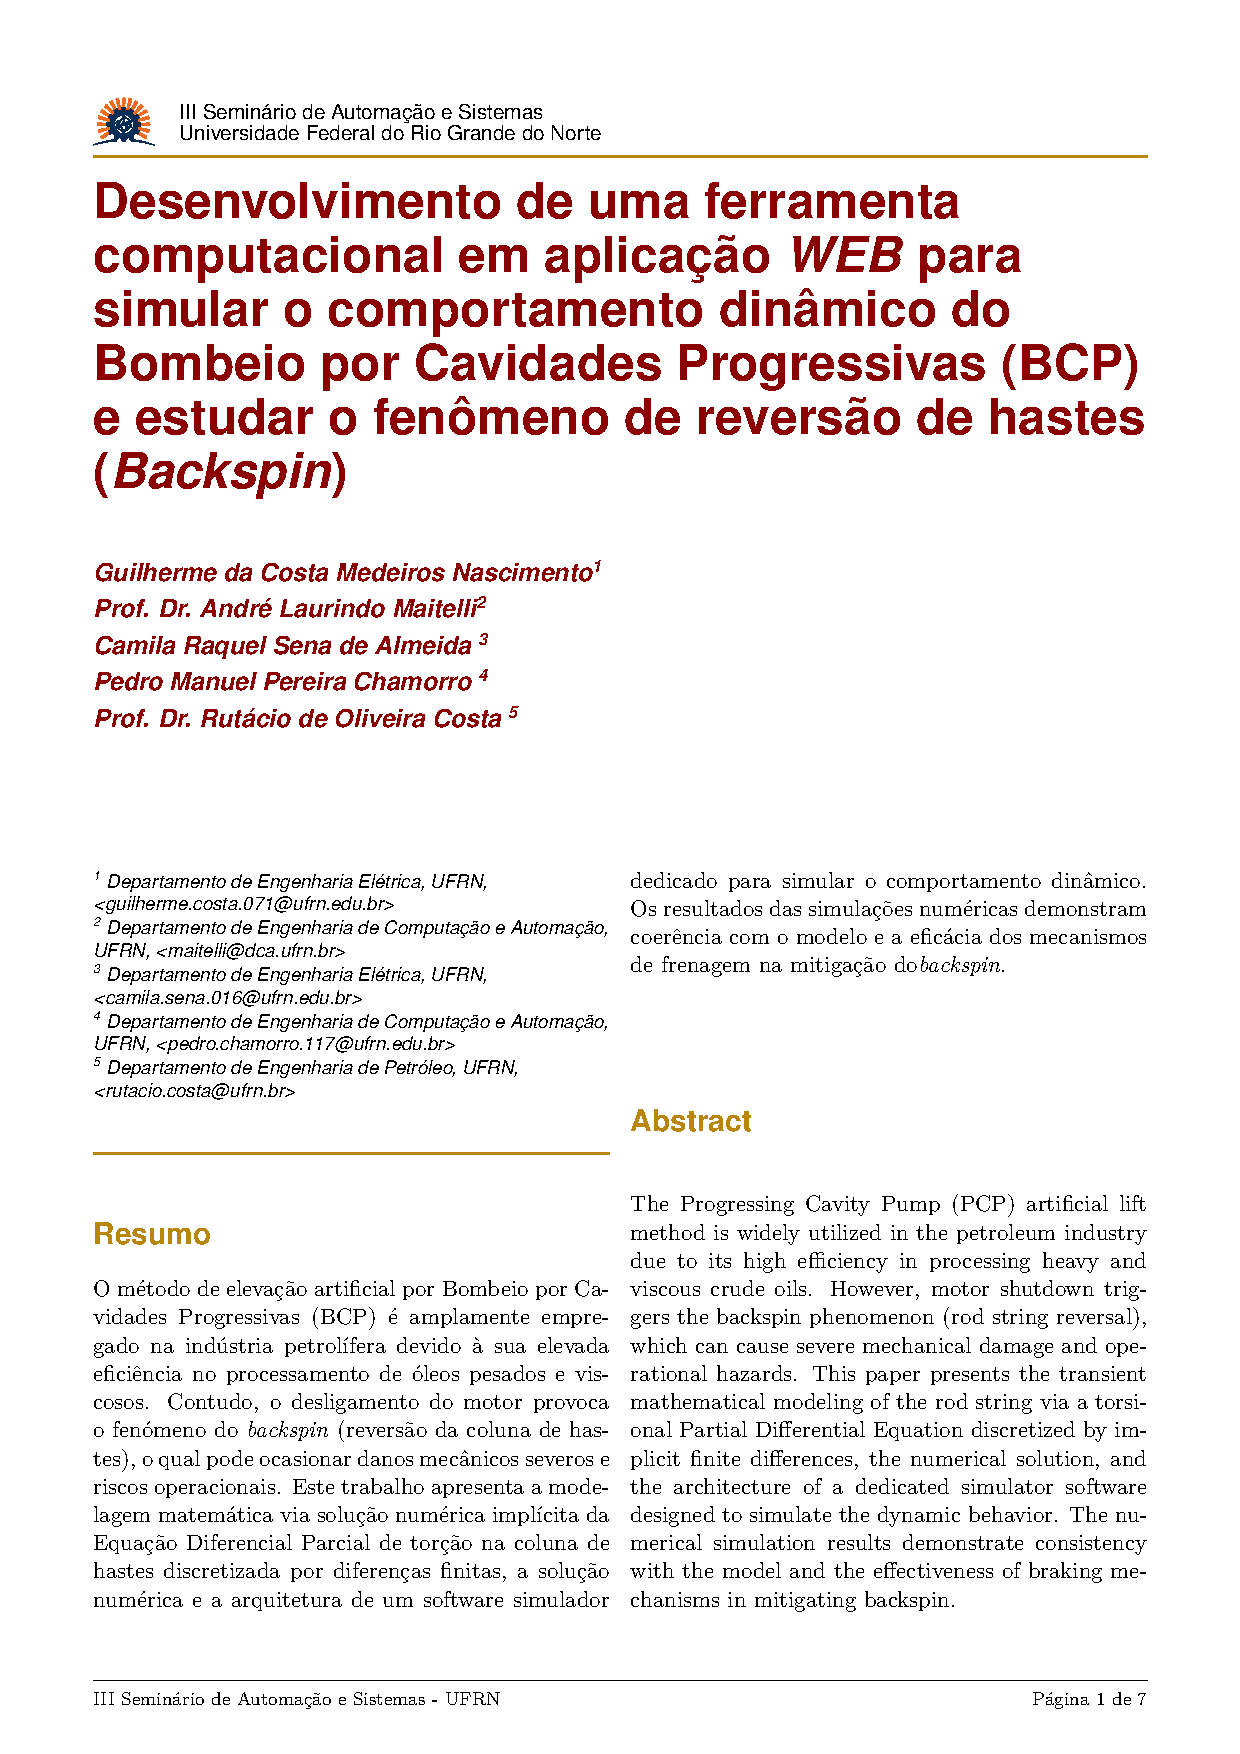
\includepdf[pages=-,fitpaper=A4]{artigos/18_desenvolvimento_de_uma_ferramenta_computacional_em_aplicacao_web_para_simular_o_comportamento_dinamico_do_bombeio_por_cavidades_progressivas_bcp_e_estudar_o_fenomeno_de_reversao_d.pdf}
\addcontentsline{toc}{section}{Desenvolvimento de uma ferramenta computacional em aplicação web para simular o comportamento dinâmico do bombeio por cavidades progressivas (BCP) e estudar o fenômeno de reversão do fluxo}

% -------------------------------------------------
% Elementos pós-textuais
% -------------------------------------------------
\backmatter
\chapter*{Índice de autores}
\addcontentsline{toc}{chapter}{Índice de autores}

% Inserir índice alfabético de autores após a definição dos artigos.
\begin{itemize}
  \item Sobrenome, Nome -- página a definir.
\end{itemize}

\chapter*{Expediente}
\addcontentsline{toc}{chapter}{Expediente}

\noindent\textbf{III Simpósio de Automação em Sistemas -- III SAS}\\
12 e 13 de novembro de 2026 -- Natal/RN\\
Organização: Laboratório de Automação (LAUT), DCA/UFRN.\\

\vspace{0.5cm}
\noindent Anais organizados pela Comissão Técnica do III SAS.\\
\noindent ISBN: a definir.\\
\noindent Editoração: a definir.\\
\noindent Apoio: FUNPEC, Idus Inteligência, eSIG Group, Centro de Tecnologia, DCA, Laut.\\

\end{document}
